%Option twoside zur Optimierung für beidseitigen Druck
\documentclass[12pt,ngerman,numbers=noenddot,abstract=true,version=first,headsepline]{scrreprt}
\renewcommand{\familydefault}{\sfdefault}
\usepackage[T1]{fontenc}
\usepackage[utf8]{inputenc}
\usepackage{geometry}
\geometry{verbose,tmargin=2.5cm,bmargin=2.5cm,head=35pt}
\setlength{\parskip}{\medskipamount}
\setlength{\parindent}{0pt}
\usepackage{array}
\usepackage{float}
\usepackage{textcomp}
\usepackage{multirow}
\usepackage{amsmath}
\usepackage{amsthm}
\usepackage{graphicx}
\usepackage{setspace}
\usepackage{microtype}
\usepackage{nomencl}
\usepackage[style=super, nopostdot, nonumberlist, nogroupskip, acronyms]{glossaries}

\makeglossaries 
\newglossaryentry{latex}
{
    name=LaTeX,
    description= {Markuplanguage für die Erstellung von wissenschaftlichen Berichten}
}
\newacronym{mes}{MES}{Manufacturing Execution System}
\newacronym{emes}{E-MES}{Enisco Manufacturing Execution System}
\newacronym{mcc}{MCC}{Manufacturing Control Cloud}
\newacronym{rest}{REST}{Representational State Transfer}
\newacronym{qos}{QoS}{Quality of Service}
\newacronym{nlp}{NLP}{Natural Language Processing}
\newacronym{dry}{DRY}{Don't Repeat Yourself}
\newacronym{tf-idf}{TF-IDF}{Term Frequency - Inverse Document Frequency}
\newacronym{tf}{TF}{Term Frequency}
\newacronym{idf}{IDF}{Inverse Document Frequency}
\newacronym{scada}{SCADA}{Supervisory Control and Data Acquisition}
\newacronym{pcs}{PCS}{Process Control System}
\makenomenclature

\setstretch{1.2}

\makeatletter

% verschieden Symbole, Zeichen wie (c), €
\usepackage{textcomp,units}

% Mehr Platz zwischen Tabelle und Untertitel
\usepackage{caption}
\captionsetup[table]{skip=10pt}

%Kapitelzahl sehr groß
\makeatletter% siehe De-TeX-FAQ 
    \renewcommand*{\chapterformat}{% 
    \begingroup% damit \unitlength-Änderung lokal bleibt 
    \setlength{\unitlength}{1mm}% 
    \begin{picture}(10,10)(0,5) 
        \setlength{\fboxsep}{0pt} 
        %\put(0,0){\framebox(20,40){}}% 
        %\put(0,20){\makebox(20,20){\rule{20\unitlength}{20\unitlength}}}% 
        \put(10,15){\line(1,0){\dimexpr 
            \textwidth-20\unitlength\relax\@gobble}}% 
        \put(0,0){\makebox(10,20)[r]{% 
            \fontsize{28\unitlength}{28\unitlength}\selectfont\thechapter 
            \kern-.05em% Ziffer in der Zeichenzelle nach rechts schieben 
            }}% 
        \put(10,15){\makebox(\dimexpr 
            \textwidth-20\unitlength\relax\@gobble,\ht\strutbox\@gobble)[l]{% 
            \ \normalsize\color{black}\chapapp~\thechapter\autodot 
            }}% 
        \end{picture} % <-- Leerzeichen ist hier beabsichtigt! 
    \endgroup 
}

\usepackage{ %a4wide,
            ellipsis, mparhack, %Fehlerkorrektur für Marginalien
            booktabs, longtable %schönere Tabellen
}


%Kurzfassung und Abstract (englisch) auf eine Seite
\renewenvironment{abstract}{
    \@beginparpenalty\@lowpenalty
    \begin{center}
    \normalfont\sectfont\nobreak\abstractname
    \@endparpenalty\@M
    \end{center}
}{
    \par
}

% schönerer Blocksatz!!
\usepackage{ifpdf} % part of the hyperref bundle
\ifpdf % if pdflatex is used 

%set fonts for nicer pdf view
\IfFileExists{lmodern.sty}{\usepackage{lmodern}}
    {\usepackage[scaled=0.92]{helvet}
    \usepackage{mathptmx}
    \usepackage{courier} }
\fi

% the pages of the TOC are numbered roman
% and a pdf-bookmark for the TOC is added
\pagenumbering{roman}
\let\myTOC\tableofcontents
\renewcommand\tableofcontents{
%\pdfbookmark[1]{Contents}{}
\myTOC
\clearpage
\pagenumbering{arabic}}

%Bezeichungen anpassen
%Babelpaket muß zuvor geladen werden
\usepackage[ngerman]{babel}
\addto\captionsngerman{ 
    \renewcommand{\figurename}{Abb.}% 
    \renewcommand{\tablename}{Tab.}% 
    \renewcommand{\abstractname}{Kurzfassung}
    \renewcommand{\nomname}{Abkürzungsverzeichnis}
}

%mehr Platz zwischen Überschrift und Tabelle
\newcommand{\@ldtable}{}
    \let\@ldtable\table
\renewcommand{\table}{ %
    \setlength{\@tempdima}{\abovecaptionskip} %
    \setlength{\abovecaptionskip}{\belowcaptionskip} %
    \setlength{\belowcaptionskip}{\@tempdima} %
    \@ldtable}

%Config für Programmcode
\usepackage{listings}
\usepackage{color}
\usepackage{scrhack}

\renewcommand{\lstlistlistingname}{Programm-Listings}

\definecolor{dkgreen}{rgb}{0,0.6,0}
\definecolor{gray}{rgb}{0.5,0.5,0.5}
\definecolor{mauve}{rgb}{0.58,0,0.82}

\lstset{frame=tb,
    language=Java,
    aboveskip=3mm,
    belowskip=3mm,
    showstringspaces=false,
    columns=flexible,
    basicstyle={\footnotesize\ttfamily},
    numbers=left,
    numberstyle=\tiny\color{gray},
    keywordstyle=\color{blue},
    commentstyle=\color{dkgreen},
    stringstyle=\color{mauve},
    breaklines=true,
    breakatwhitespace=true,
    tabsize=3
}

\AtBeginDocument{
    \def\labelitemiii{\(\circ\)}
}


\renewcommand{\author}{Moris Kotsch}
\renewcommand{\title}{Konzeption und prototypische Implementierung einer Search Engine in einer Microservice-Architektur}
\renewcommand{\subject}{Thema}
\newcommand{\keywords}{Microservices, Search Engine, Apache Kafka, Elasticsearch, Apache Solr, Full Text Search, Semantic Search}

\usepackage[automark,autooneside=false]{scrlayer-scrpage}
\clearscrheadfoot
\if@twoside
    \ofoot[\pagemark]{\pagemark}
    \ohead{\headmark}
\else
    \cfoot[\pagemark]{\pagemark}
    \ohead{
        \ifnum\value{section}>0
        \rightmark
        \fi
    }
    \ihead{
        \leftmark
    }
\fi

\makeatother

% Alle Querverweise und URLs als Link darstellen
% In der PDF-Ausgabe
\usepackage[colorlinks=true, bookmarks, bookmarksnumbered, bookmarksopen, bookmarksopenlevel=1,
    linkcolor=black, citecolor=black, urlcolor=blue, filecolor=blue,
    pdfpagelayout=OneColumn, pdfnewwindow=true,
    pdfstartview=XYZ, plainpages=false, pdfpagelabels,
    pdfauthor={\author{}}, pdftex,
    pdftitle={\title{}},
    pdfsubject={\subject{}},
    pdfkeywords={\keywords{}}]{hyperref}

\usepackage{babel}
\begin{document}
    \pagestyle{plain}
    \titlepage
\begin{center}
    \textbf{\large{}Duale Hochschule Baden-Württemberg }{\large\par}
    \par
\end{center}
\begin{center}
    \textbf{\large{}Stuttgart Campus Horb}{\large\par}
    \par
\end{center}
\begin{center}
    \begin{tabular}{l||r}
        \multicolumn{2}{c}{\vspace{1cm}}
        \tabularnewline
        \multicolumn{2}{c}{
\includegraphics[height=3.5cm]{images/dhbwlogo}}
        \tabularnewline
        \multicolumn{2}{c}{}
        \tabularnewline
        \multicolumn{2}{c}{
\includegraphics[width=0.7\textwidth, scale=1]{images/ENiscobyForcamLogo.png}}
        \tabularnewline
        \multicolumn{2}{c}{\vspace{1cm}}
        \tabularnewline
    \end{tabular}
    \par
\end{center}
\vspace{0.5cm}

\begin{flushleft}
    \textbf{\Large{}\title{}}{\Large\par}
    \par
\end{flushleft}

\begin{flushleft}
    \textbf{\textit{T3300 - Bachelorarbeit}}
    \par
\end{flushleft}

\begin{flushleft}
    {\Large{}\rule[0.5ex]{1\columnwidth}{1pt}}{\Large\par}
    \par
\end{flushleft}

\begin{tabular}{ll}
    eingereicht von:\hspace{1cm} & \author{}
    \tabularnewline
    Matrikelnummer: & 1317681
    \tabularnewline
    Kurs: & TINF2018
    \tabularnewline
    Studiengang: & Informatik
    \tabularnewline
    Hochschule: & DHBW Stuttgart Campus Horb
    \tabularnewline
    Ausbildungsfirma: & ENISCO by FORCAM GmbH
    \tabularnewline
    Ausbildungsleiterin: & Dipl.-Betriebsw. Angela Rasch
    \tabularnewline
    Unternehmen der Bachelorarbeit: & ENISCO by FORCAM GmbH
    \tabularnewline
    Betrieblicher Betreuer: & Dipl.-Ing. (FH) Franziska Simmank
    \tabularnewline
    Gutachter der DHBW: & Prof. Dr. phil. Antonius van Hoof
    \tabularnewline
    Bearbeitungszeitraum: & 07.06.2021 - 31.08.2021
    \tabularnewline
    \tabularnewline
    \multicolumn{2}{l}{Freudenstadt, \today}
    \tabularnewline
\end{tabular}
    \newpage
    
~

\vspace{17.1mm}

\begin{flushleft}
    \textbf{\huge{}Sperrvermerk}{\huge\par}
\par\end{flushleft}
Die vorliegende Praxisarbeit zum Thema \glqq Untersuchung von Analysemöglichkeiten zur Identifikation ungenutzten Codes und Features\grqq{} beinhaltet interne vertrauliche Informationen der Firma ENISCO by FORCAM GmbH. Die Weitergabe des Inhaltes der Arbeit und eventuell beiliegender Zeichnungen und Daten im Gesamten oder in Teilen ist untersagt. Es dürfen keinerlei Kopien oder Abschriften - auch in digitaler Form - gefertigt werden. Ausnahmen bedürfen der schriftlichen Genehmigung der Firma ENISCO by FORCAM GmbH.
    \newpage
    
~

\vspace{17.1mm}

\begin{flushleft}
    \textbf{\huge{}Ehrenwörtliche Erklärung}{\huge\par}
\par\end{flushleft}

Ich erkläre hiermit ehrenwörtlich:

\begin{enumerate}
    \item dass ich meine Praxisarbeit mit dem Thema \textbf{\glqq Untersuchung von Analysemöglichkeiten zur Identifikation ungenutzten Codes und Features\grqq{}} ohne fremde Hilfe angefertigt habe;
    \item dass ich die Übernahme wörtlicher Zitate aus der Literatur sowie die Verwendung der Gedanken anderer Autoren an den entsprechenden Stellen innerhalb der Arbeit gekennzeichnet habe;
    \item dass ich meine Praxisarbeit bei keiner anderen Prüfung vorgelegt habe.
\end{enumerate}

Ich bin mir bewusst, dass eine falsche Erklärung rechtliche Folgen haben wird.

\vspace{2cm}

\begin{center}
    \begin{tabular*}{\textwidth}{@{\extracolsep{\fill}}cl}
        Freudenstadt, \today & 
\includegraphics[width=0.3\textwidth]{images/Unterschrift.png}
        \tabularnewline
        & \author{}
        \tabularnewline
    \end{tabular*}
    \par
\end{center}
    \newpage
    
~

\vspace{17.1mm}

\begin{flushleft}
    \textbf{\huge{}Zusammenfassung}{\huge\par}
\par\end{flushleft}

Die vorliegende Bachelorarbeit mit dem Titel \glqq Konzeption und prototypische Implementierung einer Search Engine in einer Microservice-Architektur\grqq{}, erläutert die verschiedenen Möglichkeiten für die Umsetzung einer Suchfunktionalität. 

Die Suchfunktionalität soll in naher Zukunft in der MES-Software \glqq MCC\grqq{} eingesetzt werden. Hierbei ist \glqq MCC\grqq{} die Neugestaltung des aktuellen Produktionsleitsystems \glqq E-MES\grqq der Firma Enisco by Forcam GmbH. Bei der Neugestaltung wird von einer monolithisch betriebenen, modularen 3-Schichten-Architektur auf eine verteilte Microservice-Architektur gewechselt.

Im Rahmen dieser Arbeit wird zunächst auf die verschiedenen Arten von Suchfunktionalitäten in modernen Informationssystemen eingegangen. Dabei wird die Volltextsuche, die facettierte Suche und die semantische Suche näher betrachtet. Der jeweilige Umfang der Sucharten wird anhand des Funktionsumfangs des Produktionsleitsystems \glqq MCC\grqq{} definiert. Hierfür erfolgt eine Erläuterung des Funktionsumfangs.

Bei der Erstellung eines geeigneten Konzeptes werden gültige Architektur-Prinzipien beachtet, um monolithische Seiteneffekte bei der Einführung einer Suchfunktionalität zu vermeiden. Innerhalb des Konzeptes wird eine Auswahl bezüglich einer Search Engine und einer geeigneten Datenpipeline getroffen. Hierbei werden die Search Engines \glqq Apache Solr\grqq{} und \glqq Elasticsearch\grqq{} gegenübergestellt und bezüglich einer Datenpipeline werden die Umsetzungsmöglichkeiten \glqq Dual Write\grqq{}, \glqq Polling\grqq{} und \glqq Change-Data-Capture\grqq{} verglichen.

Im Anschluss erfolgt eine prototypische Umsetzung der Change-Data-Capture - Datenpipeline in Verbindung mit der Search Engine \glqq Elasticsearch\grqq{}.

    \newpage
    
~

\vspace{17.1mm}

\begin{flushleft}
    \textbf{\huge{}Abstract}{\huge\par}
\par\end{flushleft}

This bachelor thesis with the title \glqq Konzeption und prototypische Implementierung einer Search Engine in einer Microservice-Architektur\grqq{} explains the different possibilities for the implementation of a search functionality.

The search functionality is to be implemented in the MES software \glqq MCC\grqq{} in the near future. \glqq MCC\grqq{} is the redesign of the current production control system \glqq E-MES\grqq{} of the company Enisco by Forcam GmbH. In the redesign, a change is made from a monolithically operated, modular 3-layer architecture to a distributed microservice architecture.

In the context of this work, the different types of search functions in modern information systems will be discussed first. Full-text search, faceted search, and semantic search will be examined in more detail. The respective scope of the search types is defined on the basis of the functional scope of the production control system \glqq MCC\grqq{}. For this purpose, an explanation of the functional scope is given.

When creating a suitable concept, valid architectural principles are taken into account in order to avoid monolithic side effects when introducing a search functionality. Within the concept, a selection is made regarding a search engine and a suitable data pipeline. The search engines \glqq Apache Solr\grqq{} and \glqq Elasticsearch\grqq{} are compared, and the implementation options \glqq Dual Write\grqq{}, \glqq Polling\grqq{} and \glqq Change-Data-Capture\grqq{} are compared with regard to a data pipeline.

This is followed by a prototypical implementation of the change data capture data pipeline in conjunction with the search engine \glqq Elasticsearch\grqq{}. 

    \newpage

    \tableofcontents
    \newpage

    \pagenumbering{roman}
    %ACHTUNG: Korrekte Seitenzahl bei Fertigstellung des Dokuments einstellen, andernfalls ist die Nummerierung u.U. fehlerhaft.
    \setcounter{page}{7}

    \listoffigures
    \newpage

    %\lstlistoflistings
    %\newpage

    %\listoftables
    %\newpage

    %\printglossary[title=Abkürzungsverzeichnis, type=\acronymtype]
    %\printglossary
    %\newpage

    %asd
    %GGF anpassen
    %Index aktualisieren mit: makeindex Vorlage.nlo -s nomencl.ist -o Vorlage.nls
    %\printnomenclature[3cm]{}
    %\newpage


    \pagenumbering{arabic}
    %Kopfzeile aktivieren
    \pagestyle{headings}
    %Alle Werke ins Literaturverzeichnis
    %nocite{*}

    \chapter{Einleitung\label{chap1:Erstes-Kapitel}}

Im Rahmen der vorliegenden Arbeit werden verschiedene Umsetzungsmöglichkeiten für eine Suchfunktionalität in einem MES-Produkt der Firma Enisco betrachtet. Der Fokus liegt hierbei auf den diversen Arten für die Umsetzung einer Suche. Durch die architekturelle Neugestaltung des bisherigen MES-Produktes wird auch auf die technischen Besonderheiten bezüglich der Suchfunktionalität in einer Microservice-Architektur eingegangen.

Im folgenden, einleitenden Kapitel wird die betreuende Firma mit dem dazugehörigem Kernprodukt E-MES, die Aufgabenstellung und das geplante Vorgehen erläutert. Um das Lesen der Arbeit zu erleichtern, wird ein Überblick über den Aufbau der Arbeit gegeben.

\section{Enisco und E-MES\label{sec1.1:unterpunkt-1}}

Die vorliegende Arbeit wurde im Rahmen einer Bachelorarbeit bei der Firma Enisco verfasst. Enisco GmbH \& Co. KG wurde 2015 als Tochtergesellschaft der Eisenmann SE gegründet und ist mittlerweile ein eigenständiges Unternehmen, welches unter dem Namen \glqq Enisco by Forcam GmbH\footnote{Im Folgenden wird aus Gründen der Lesbarkeit auf die Rechtsform der Enisco by Forcam GmbH verzichtet}\grqq{} agiert.

Als Kernprodukt vertreibt die Firma Enisco das Produktionsleitsystem \glqq \gls{emes}\grqq{}. Dieses wird für die Überwachung und Steuerung von Produktionsanlagen eingesetzt. E-MES vernetzt dabei die Anlage sowohl horizontal, über den gesamten Fertigungsprozess, als auch vertikal, über alle Prozessebenen hinweg und bildet so ein System, welches zwischen Unternehmensebene (ERP, engl. für Enterprise Ressource Planning) und Steuerungsebene (PLC, engl. für Programmable Logic
Controller) agiert. \cite{EniscobyForcamGmbH.2021b}

E-MES ist dafür modular aufgebaut und besitzt als Basis ein Platform-Modul. Dieses beinhaltet alle Grundlagen und Schnittstellen für die Installation weiterer Module. Die zusätzlichen Module (engl. Add-Ons) ergänzen E-MES um bestimmte Funktionen und können kundenspezifisch installiert und konfiguriert werden.

\section{Aufgabenstellung\label{sec1.2:Unterpunkt-2}}

Derzeit erfährt das aktuelle Produktionsleitsystem E-MES eine Neugestaltung. Dabei wird von einer monolithisch betriebenen, modularen 3-Schichten-Architektur auf eine verteilte Microservice-Architektur gewechselt. Ein Wechsel der Architektur beruht auf dem Eintritt der Muttergesellschafft Forcam GmbH in die \glqq Open Industry 4.0 Alliance\grqq{}. Durch den Zusammenschluss von mehreren Unternehmen aus dem Bereich \glqq Industrie 4.0\grqq{} können einheitliche Schnittstellen definiert werden, um so die Interoperabilität zwischen den Softwarelösungen der beteiligten Firmen zu stärken \cite{OpenIndustry4.0Alliance.2021}. Um die benötigte Interoperabilität zu ermöglichen, setzen die beteiligten Unternehmen vermehrt auf Technologien wie Docker und Kubernetes. Um nun auch die Neugestaltung von E-MES in diesem Umfeld anzubieten, wurde sich für eine verteilte Microservice-Architektur entschieden. Neben der Architektur wird auch der Produktname von \glqq E-MES\grqq{} in den vorläufigen Produktnamen \glqq \gls{mcc}\grqq{} abgeändert.

Im Zuge der Neugestaltung von E-MES werden neue Funktionalitäten, wie eine Suchfunktion integriert. Eine Suchfunktion in modernen Informationssystemen wird von den Benutzern als gewohnter Komfort wahrgenommen. Für die Umsetzung einer Suchfunktion in einem \gls{mes} muss festgelegt werden, welche Funktionen und Inhalte des \gls{mes} von der Suchfunktion abgedeckt werden sollen. Neben der Suche nach Funktionalitäten des Systems, kann es auch hilfreich sein, nach bestimmten \glqq Objekten\grqq{} innerhalb des Systems zu suchen. Solche Objekte können zum Beispiel in Form von eindeutigen Aufträgen oder Maschinen in einem \gls{mes} vorkommen. Gibt der Benutzer die Kennung eines Objektes in das Suchfeld ein, sollen ihm alle Funktionen und Informationen bezüglich dieses Objektes angezeigt werden. So soll der Benutzer bei der Navigation durch das \gls{mes} unterstützt werden.

Neben der Anforderungsklärung bezüglich der Suchoptionen und der Granularität der Suchanfragen, gilt es auch eine Konzeption für die Integration einer Search Engine in die MCC-Gesamtarchitektur zu entwerfen. Hierbei sind die besonderen Anforderungen zu beachten, welche durch die Einführung der verteilten Microservice-Architektur entstanden sind. So ist zu klären, welche Strategie für die Datenaktualisierung zwischen einer Search Engine und den Datenhaltungsschichten der einzelnen Services den Anforderungen am besten entspricht. Anhand von selbstgewählten technischen und lizenzbezogenen Kriterien sollen diesbezüglich Strategien und auch potentiell geeignete Search Engines verglichen werden. Bei der Konzeption für die Integration einer Search Engine sind monolithische Seiteneffekte, die durch die Missachtung von Prinzipien der Microservice-Architektur entstehen könnten, zu vermeiden.

Das erstellte Konzept gilt es anschließend mithilfe einer prototypischen Implementierung einer Suchanwendung als \glqq Proof of Concept\grqq{} umzusetzen.

\section{Vorgehensweise und Aufbau der Arbeit\label{sec1.3:Unterpunkt-3}}

Die Vorgehensweise und die schriftliche Ausarbeitung der vorliegenden Arbeit gliedert sich in drei Hauptteile. Als Vorarbeit für die eigentliche Bearbeitung werden in \textbf{\autoref{chap2:Zweites-Kapitel}} die theoretischen Grundlagen über die verschiedenen Umsetzungsmöglichkeiten einer Suchfunktion erläutert. Durch die Erläuterung von allgemeingültigen Architektur-Prinzipien und im spezielleren Anti-Pattern der Microservice-Architektur, werden die theoretischen Grundlagen für die Vermeidung von monolithischen Seiteneffekten geschaffen.

Im ersten Teil der Arbeit wird definiert, mit welchem Suchumfang die Search Engine innerhalb von \gls{mcc} nach Funktionen und Objekten agieren soll. Da zum Zeitpunkt der Erstellung dieser Arbeit noch keine produktreife Version von \gls{mcc} existiert, wird sich an dem Produktumfang und den Funktionalitäten des aktuellen Produktes \gls{emes} orientiert. In \textbf{\autoref{chap3:Drittes-Kapitel}} wird der Suchumfang für die Suchfunktionalität definiert. Hierbei wird bei \gls{mcc} analysiert, welche Objekte innerhalb des Systems \glqq suchbar\grqq{} gemacht werden sollen.

Ein weiterer Schritt ist die Konzeption für die Integration einer Search Engine in \gls{mcc}. Es werden hierbei in \textbf{\autoref{chap4:Viertes-Kapitel}} verschiedene Search Engines anhand von technischen und lizenzbezogenen Kriterien miteinander verglichen. Ebenso werden verschiedene Umsetzungsmöglichkeiten der Datenaktualisierung zwischen einer Search Engine und den Datenhaltungsschichten der einzelnen Services erläutert und anhand von Vergleichskriterien miteinander verglichen. Vorbereitend für die prototypische Umsetzung wird zusätzlich ein Gesamtkonzept erstellt.

Anschließend an die Konzeption folgt in \textbf{\autoref{chap5:Fuenftes-Kapitel}} eine Beschreibung der prototypischen Umsetzung anhand einer Proof-of-Concept-Anwendung. Hierfür wird zunächst festgelegt, welchen Umfang jene prototypische Umsetzung besitzen soll und ob bereits Softwareteile aus \gls{mcc} verwendet werden können.

Abgeschlossen wird die Arbeit in \textbf{\autoref{chap6:Sechstes-Kapitel}} mit einer Zusammenfassung der gewonnen Erkenntnisse und mit einem Ausblick auf die spätere Integrierung in das Produktionsleitsystem MCC.
\chapter{Grundlagen\label{chap2:Zweites-Kapitel}}

Grundlegend wird in folgendem Kapitel auf den Funktionsumfang von Suchfunktionalitäten in modernen Informationssystemen eingegangen. Differenziert wird dabei betrachtet, inwiefern sich die Anforderungen an eine Suchfunktionalität zwischen einer Websuche, einer Suche in einem E-Commerce - Shop und einer Suche in einem MES-System unterscheiden. Neben den Anforderungen und Charakteristiken der Suchfunktionen, werden auch die verschiedenen Umsetzungsmöglichkeiten \glqq Volltextsuche\grqq{}, \glqq Facetten-Suche\grqq{} und \glqq semantische Suche\grqq{} erläutert. Für eine nach Relevanz sortierte Auflistung der Suchergebnisse, wird eine Möglichkeit der Relevanzbestimmung vorgestellt.

% Neben einer Klärung, welchen Mehrwert eine Suchfunktionalität liefert, werden auch die Umsetzungsmöglichkeiten \glqq Volltextsuche\grqq{}, \glqq Facetten-Suche\grqq{} und \glqq semantische Suche\grqq{} aufgezeigt. Ergänzend wird die Relevanzbestimmung von Suchtreffern thematisiert.

Um eine Konzeption und prototypische Umsetzung einer Volltextsuche in \gls{mcc} zu ermöglichen, wird in zusätzlich auf die architekturellen Hintergründe von \gls{mcc} eingegangen. Hierfür werden zu Beginn allgemein gültige Architektur-Prinzipien erläutert, welche auch bei der Integration einer Volltextsuche berücksichtigt werden müssen und somit bei der Auswahl eines geeigneten Konzeptes von Bedeutung sind.

Aufbauend auf den Architektur-Prinzipien wird die verwendete Microservice-Architektur erläutert, wobei neben einer allgemeinen Einführung in die Architektur auch auf die Kommunikation von Microservices untereinander eingegangen wird. Um mögliche Fehlkonzeptionen zu vermeiden, werden häufig auftretende Anti-Pattern aufgezeigt, welche unter Umständen zu monolithischen Seiteneffekten führen können.

\section{Suchfunktionen in modernen Informationssystemen\label{sec2.1:Unterpunkt-1}}

Aufgrund der fortlaufenden Digitalisierung und Themen wie \glqq Industrie 4.0\grqq{} und \glqq Internet of Things\grqq{} steigt die jährlich anfallende Datenmenge im weltweiten Internet. Das aufkommende Datenvolumen wird bereits für das Jahr 2025 auf 175 Zettabyte prognostiziert \cite{F.Tenzer.2018}. Dies wäre ein Wachstum, vom Jahr 2018 bis zum Jahr 2025, um mehr als den Faktor fünf.

Neben den reinen Daten wachsen zunehmend auch die Anzahl der Websites und Web-Inhalten. So gibt es Stand 2021 rund 1,83 Milliarden Websites \cite{GuyFawkes.2021}, welche durch Suchmaschinen, wie Google gefunden werden können. Ein Nutzer kann hierbei einen Volltext als Sucheingabe eingeben und erhält eine Liste mit den entsprechenden Treffern sortiert nach der Relevanz für den Nutzer. Solche Suchfunktionalitäten werden auch direkt auf den Websites angeboten, um den Besuchern so das Navigieren durch die Website und das Auffinden von Produkten und Dienstleistungen zu erleichtern.

% Nach einer Studie des eCommerce-Leitfadens \cite{AaronSchrettenbrunner.} geben 80\% der Shopbesitzer an, dass die Suchfunktion auf ihrer Website ihnen \glqq sehr wichtig\grqq{} ist. Demnach geben 97\% der Befragten an, dass sie eine Suchfunktion im Shop anbieten.

Je nach Art der Benutzer und Umfang der Produkte und Informationen stehen bei der Umsetzung einer Suchfunktion zwei Möglichkeiten zur Verfügung. Eine Möglichkeit ist die Suche mit Hilfe einer Volltextsuche. Für einen Benutzer stellt solch eine Art der Suchfunktion einen bekannten Komfort dar, da diese Art bereits aus Web-Suchmaschinen, wie zum Beispiel Google bekannt ist. Eine weitere Möglichkeit bietet die Suche über verschiedene Filter. Hierbei werden die Details der Informationen über verschiedene Facetten definiert. Durch Filterung der Facetten können dann die Informationen gefunden werden.

Als Ergänzung zur Volltextsuche und facettierten Suche wird bei der semantischen Suche zusätzlich noch der semantische Wert einer Suchanfrage berücksichtigt. Dadurch ist es möglich dem Benutzer der Suchfunktionalität relevante Suchergebnisse zu liefern.

\subsection{Anwendungsgebiete für Suchfunktionen\label{subsec2.1.1:Unterunterpunkt-1}}

Je nach Anwendungsgebiet einer Suchfunktionalität gibt es Unterschiede bezüglich dem Umfang des suchbaren Datenkontextes und der Größe des Benutzerkreises. Aufgrund dieser Unterschiede ist eine passende Auswahl beziehungsweise Kombination der Umsetzungsmöglichkeiten für die Suchfunktionalitäten von Nöten. Anschließend an die Betrachtung von den drei Anwendungsgebieten \glqq Websuche\grqq{}, \glqq E-Commerce - Suche\grqq{} und \glqq MES-Suche\grqq{}, werden die Umsetzungsmöglichkeiten näher erläutert.

Ein Anwendungsgebiet ist die Websuche, bei welcher explizit nach Websites und den Web-Inhalten gesucht wird. Hierbei stellt das World Wide Web den Datenkontext dar und ist aufgrund der Größe von rund 1,83 Milliarden Websites (Stand 2021) \cite{GuyFawkes.2021} nicht mehr ohne Suchmaschinen, wie zum Beispiel Google, zu durchsuchen. Umgesetzt wird die Suchfunktionalität bei der Websuche durch die Verwendung einer Volltextsuche. Um den Benutzern effektivere Suchtreffer zu gewährleisten, wird bei Suchmaschinen, wie Google, zusätzlich noch eine semantische Suche verwendet.

Auch in Online-Shops beziehungsweise E-Commerce - Shops ist eine Suchfunktion für die Navigation innerhalb der Websites von Nöten. Der durchsuchbare Datenkontext ist abhängig vom  angebotenem Artikelumfang der Website. Eine Suchfunktion ist im Gegensatz zur Websuche nicht unbedingt notwendig, da Produkte und Dienstleistungen auch durch eine Navigation durch die Website erreichbar sind. Jedoch ist der Benutzerkreis oftmals nicht mit dem Aufbau der Website vertraut, so dass eine Suchfunktionalität bei der Navigation innerhalb der Website unterstützen kann. Oft zu finden ist eine Kombination aus einer Volltextsuche und einer facettierten Suche. Hierbei wird dem Benutzer primär eine Volltextsuche in Form eines Eingabefeldes angeboten und anschließend kann über eine \glqq Erweiterte Suche\grqq{} die Facettierung vorgenommen werden. Ein bekanntes Beispiel für die Verwendung einer Kombination beider Möglichkeiten ist der Onlineversandhändler \glqq Amazon\grqq{}. Durch die Eingabe eines Suchbegriffes wird dem Benutzer eine Auswahl geeigneter Suchtreffer angezeigt. Für eine weitere Eingrenzung der Suchergebnisse kann der Benutzer die Ergebnisse zum Beispiel anhand der Preise, Bewertungen oder Hersteller filtern.

Im Rahmen dieser Arbeit wird explizit die Einführung einer Suchfunktionalität in ein MES-System betrachtet. Der Datenkontext eines MES-Systems kann hierbei sowohl ein großes Volumen als auch eine hohe Komplexität aufweisen. Je nach Funktionsumfang und Struktur des MES-Systems kann auch die Navigation innerhalb des Systems erschwert sein. Der überwiegend explizite Benutzerkreis muss daher im Umgang mit dem MES-System geschult werden. Damit sowohl neuen Benutzern der Umgang mit dem System ermöglicht, und erfahrenen Benutzern der Umgang mit dem System erleichtert wird, kann eine Kombination aus Volltextsuche und facettierter Suche verwendet werden.

% \subsection{Mehrwert einer Suchfunktion\label{subsec2.1.1:Unterunterpunkt-1}}

% Der Mehrwert bei der Einführung einer Suchfunktion in einer Website oder in einem Software-Produkt, wie \gls{mcc}, liegt bei der Unterstützung der Benutzer beim Navigieren und Auffinden von Produkten oder Dienstleistungen.

% Aufgrund der wachsenden Anzahl der Websites und Web-Inhalten \cite{GuyFawkes.2021} ist ein eigenständiges Navigieren durch das World Wide Web nicht mehr möglich. Durch die Verwendung von Suchmaschinen können Benutzer mit beliebigen Suchbegriffen nach expliziten Websites oder Web-Inhalten suchen.

% Der Benutzerkreis von Software-Produkten, wie \gls{mcc}, besteht überwiegend aus einem expliziten Benutzerkreis. Im Umfeld von \gls{mcc} sind dies vor allem die Betreiber der jeweiligen Anlagen. Damit sich auch neue und unerfahrene Benutzer in einer solchen umfangreichen Software zurechtfinden, kann eine Suchfunktionalität den Einstieg erleichtern. So kann der Produktumfang von \gls{mcc} benutzt werden, ohne die genaue Struktur und den kompletten Funktionsumfang zu kennen.

\subsection{Volltextsuche\label{subsec2.1.2:Unterunterpunkt-2}}

Eine Möglichkeit nach Produkten oder Informationen zu suchen, ist die Volltextsuche. Hierbei kann der Benutzer einen beliebigen Freitext in ein Suchfeld eingeben und erhält eine Auflistung der Suchtreffer, welche den eingegebenen Freitext enthalten.

Da auch Suchmaschinen wie Google auf einer Volltextsuche basieren, ist diese Art der Suchfunktion, für die Benutzer ein gewohnter Komfort. Eine Volltextsuche wird dabei nicht nur in den Suchmaschinen oder direkt in auf den Websites angeboten, sondern auch für die Navigation und Suche in Software-Produkten. Ein Beispiel hierfür ist die Wiki-Software \glqq Atlassian Confluence\grqq{}, welche standardmäßig eine Suchfunktion zur Verfügung stellt. Für die Wissensaufnahme und Weitergabe der Firma Enisco wird diese Wiki-Software verwendet.

In \autoref{fig:search_confluence_fulltextsearch} ist beispielhaft die Trefferauflistung des Suchbegriffes \glqq Studenten\grqq{} abgebildet. Hierbei dursucht die Suchfunktion den Datenbestand der Confluence-Anwendung der Firma Enisco und gibt als Ergebnis alle Seiten zurück, welche mit dem Suchbegriff übereinstimmen. In der gezeigten Ansicht erscheinen dabei alle Seiten, welche einen Treffer im Titel aufweisen. Durch die Schaltfläche \glqq Suche nach \textbf{Studenten}\grqq{}, welche in der Ansicht unten angezeigt wird, werden auch Confluence-Seiten angezeigt, in welchen der Suchbegriff auch im eigentlichen Inhalt der Seite gefunden wird.

\begin{figure}[H]
    \centering
    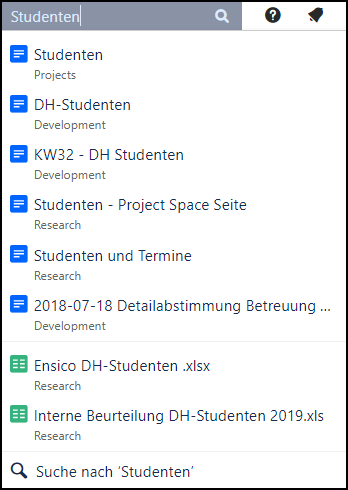
\includegraphics[width=0.4\linewidth]{images/Suchleiste_Confluence.png}
    \caption{Ergebnisse der Suchanfrage \glqq Studenten\grqq{} - entnommen aus \cite{EniscobyForcamGmbH.2021}\protect\footnotemark}
    \label{fig:search_confluence_fulltextsearch}
\end{figure}

\footnotetext{Quelle aus dem Intranet (nicht öffentlich zugänglich) von der Enisco by Forcam GmbH}

Grundlage für die technische Umsetzung einer Volltextsuche ist die Erstellung eines Suchindexes. Ein Suchindex für die Volltextsuche wird hierbei als invertierter Index umgesetzt \cite{SebastianRuss.2017}. Die Funktionsweise von einem invertierten Index ist vergleichbar mit dem Stichwortverzeichnis in Büchern. Bei der Suche nach einem bestimmten Wort oder Begriff in Büchern, ist eine Suche durch das gesamte Buch umständlich und mit einem hohen Zeitaufwand verbunden. Durch die Verwendung eines Stichwortverzeichnis, wie in \autoref{fig:inverted_index} abgebildet, werden die Begriffe aus dem Buch den einzelnen Seiten zugewiesen. Eine Suche im Stichwortverzeichnis ist aufgrund der Vorsortierung schneller und man kann direkt an die entsprechende Stelle im Buch springen.

\begin{figure}[H]
    \centering
    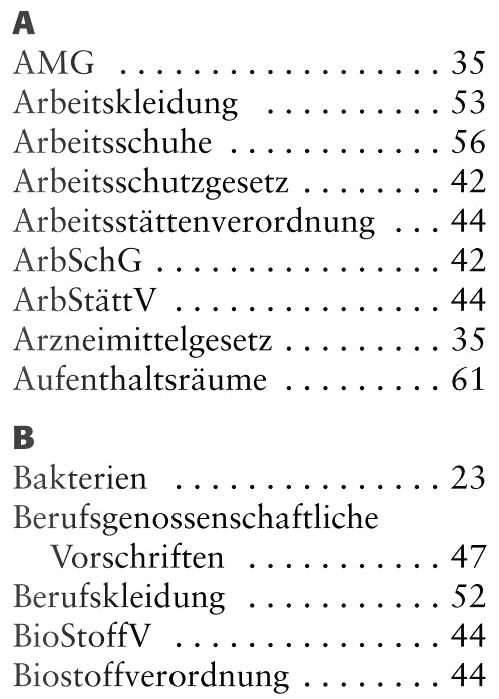
\includegraphics[width=0.3\linewidth]{images/Stichwortverzeichnis.png}
    \caption{Beispiel für ein Stichwortverzeichnis \cite{weka.de.2014}}
    \label{fig:inverted_index}
\end{figure}

Bei der Eingabe von Freitexten durch menschliche Benutzer ist das Aufkommen von Fehleingaben nicht auszuschließen. Aus diesem Grund müssen sowohl beim Aufbau des invertierten Indexes, als auch beim Bearbeiten der Suchanfrage gewisse Transformationsschritte berücksichtigt werden \cite{SebastianRuss.2017}. Die Transformationsschritte sorgen für eine Fehlertoleranz innerhalb der Suchfunktion und verbessern die User Experience bezüglich der Benutzung der Suchfunktion.

Die Transformationsschritte werden benötigt, um die Vielzahl der unterschiedlichen Suchanfragen korrekt zu beantworten \cite{SebastianRuss.2017}. Hierbei werden je nach Anforderungen verschiedene Tokenizer und Analyzer verwendet. In \autoref{fig:index_analyzer} ist eine beispielhafte Abfolge von Transformationsschritten aufgezeigt. Ziel ist es, die variantenreiche Suchphrase durch eine Normalisierung in ein einheitliches Format zu überführen. Dadurch kann eine ausreichende Fehlertoleranz geschaffen werden. Neben der Suchphrase müssen die Transformationsschritte auch bei der Erstellung des Indexes berücksichtigt werden \cite{SebastianRuss.2017}.

Die in \autoref{fig:index_analyzer} aufgezeigten Transformationsschritte werden nachfolgend näher erläutert.

\begin{figure}[H]
    \centering
    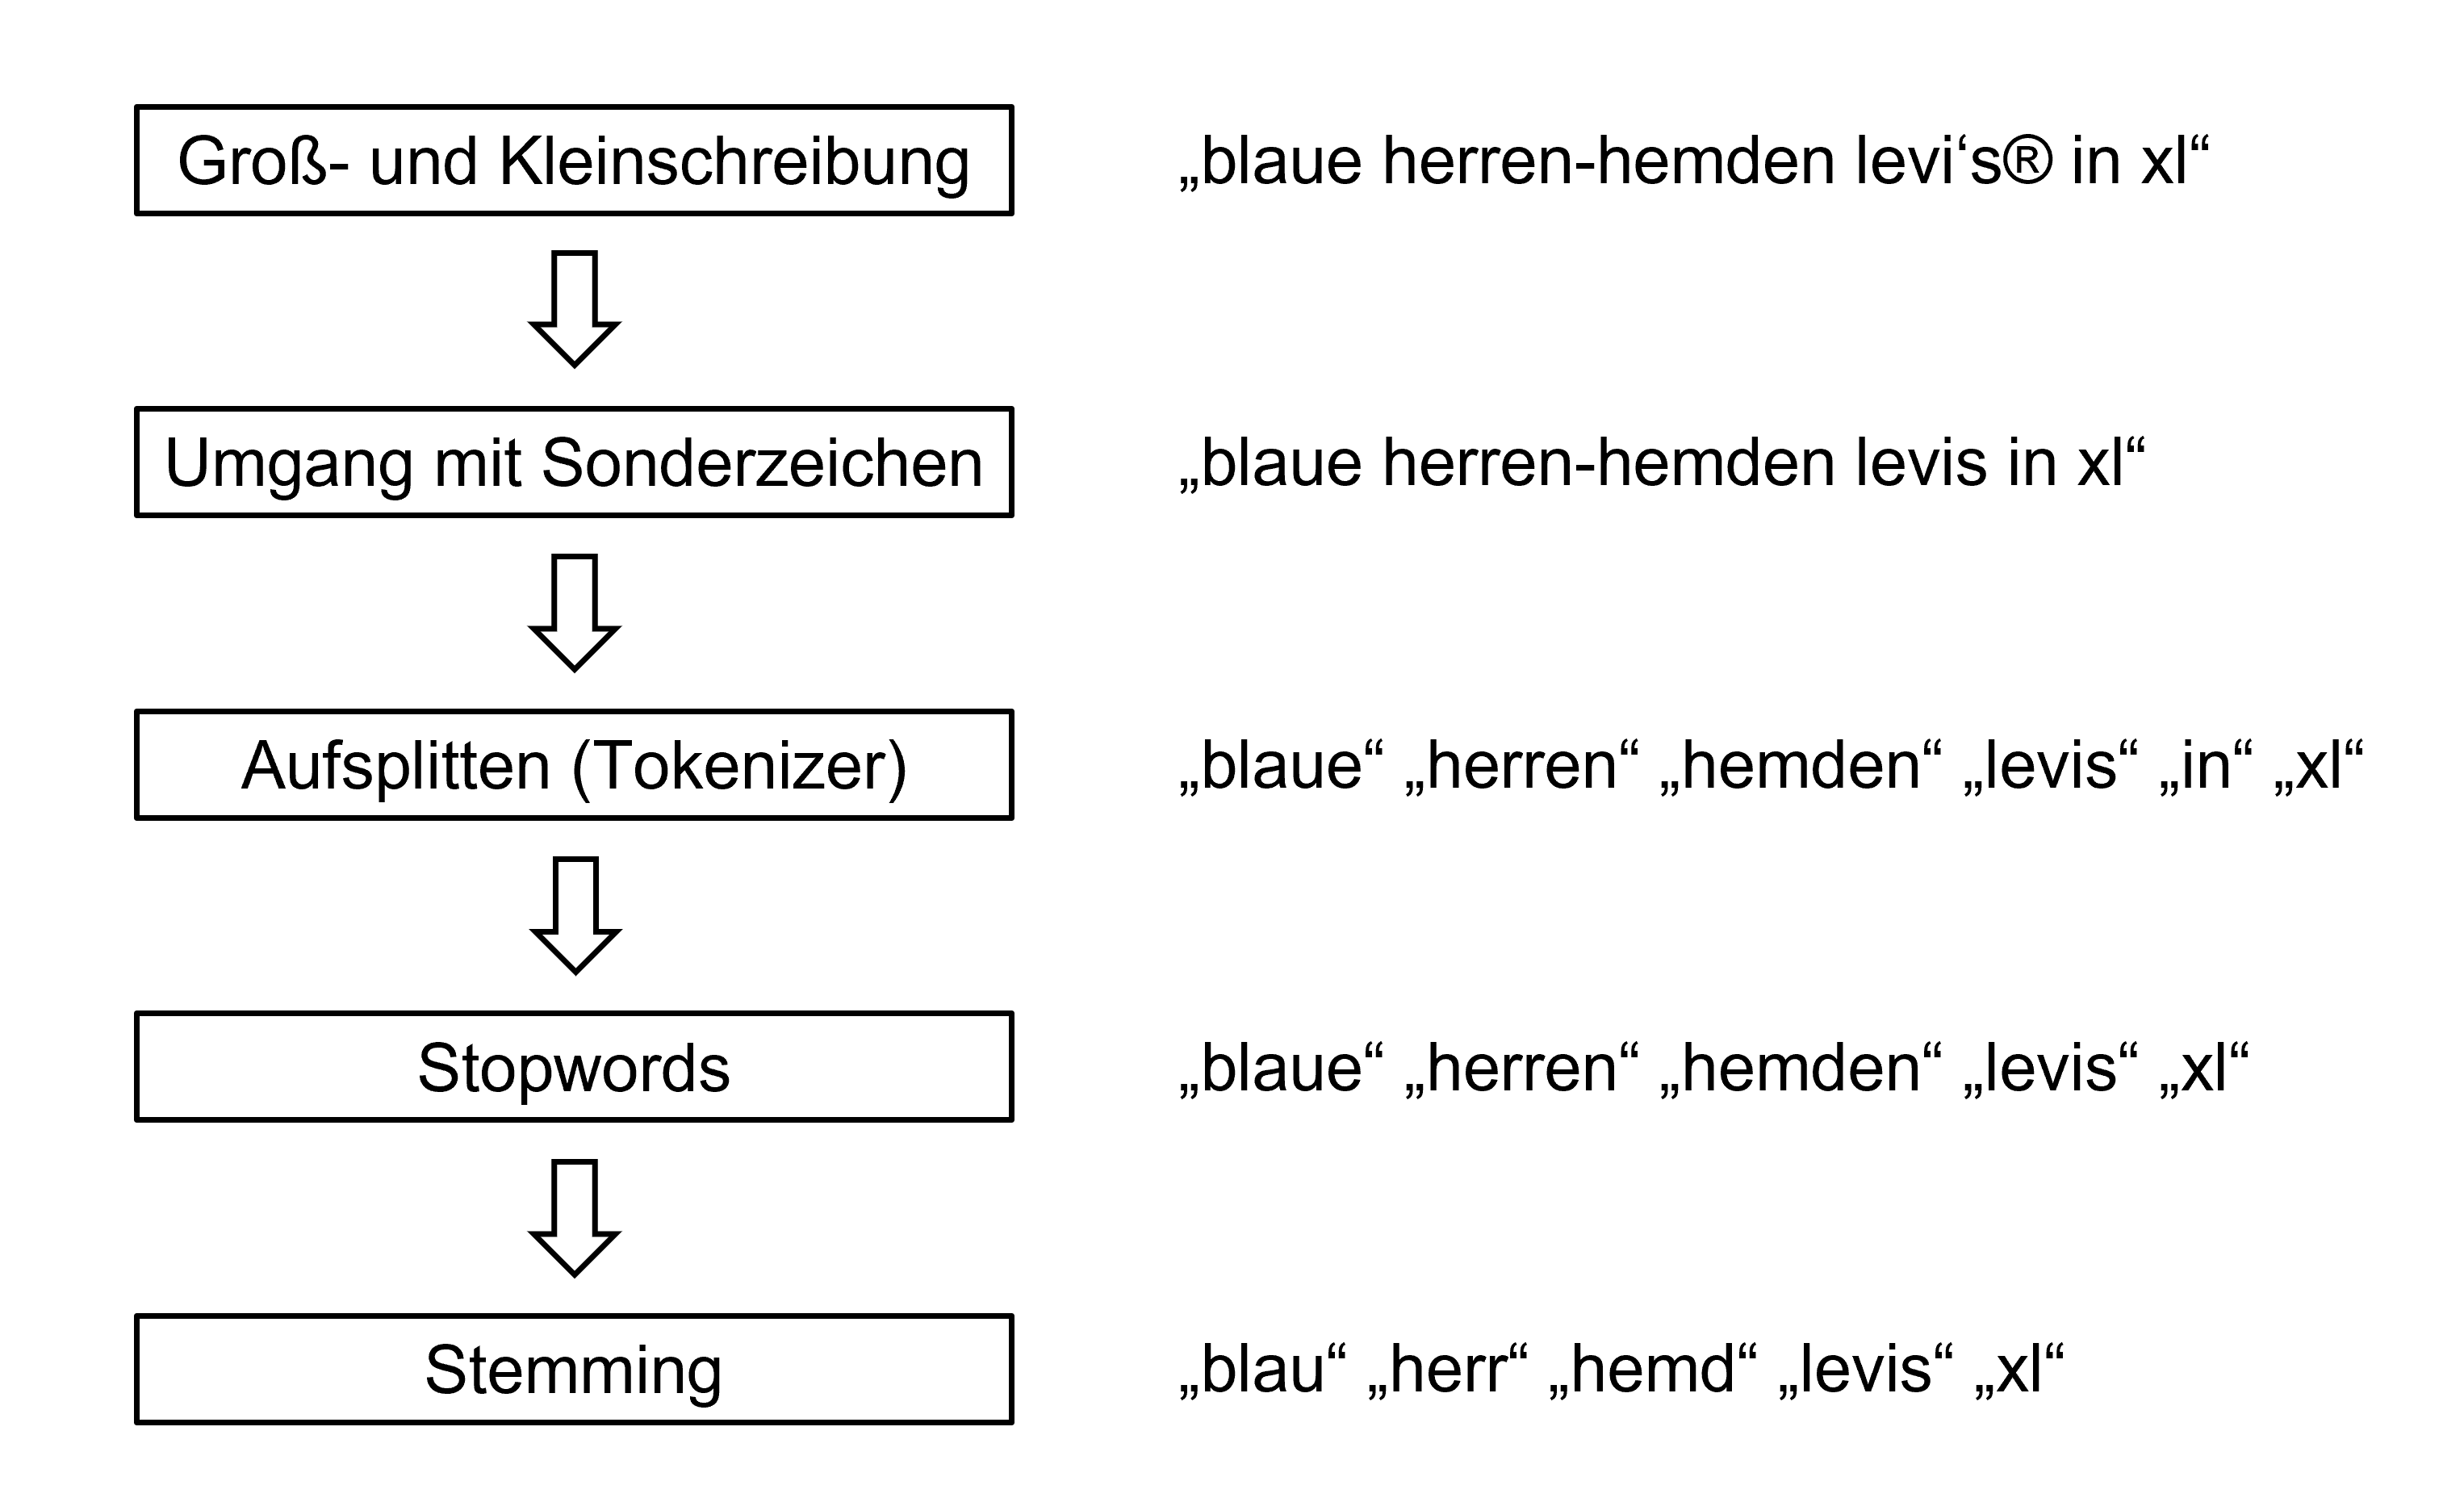
\includegraphics[width=0.65\linewidth]{images/Index_Analyzer.png}
    \caption{Beispielhafter Ablauf der Transformationsschritte - in Anlehnung an \cite{SebastianRuss.2017}}
    \label{fig:index_analyzer}
\end{figure}

\subsubsection{Tokenizer}

Hierbei wird die komplette Suchphrase in verschiedene Suchbegriffe (auch Tokens genannt) aufgeteilt. So wird beispielsweise aus der Suchphrase \glqq Hose Blau\grqq{} die Tokens \glqq Hose\grqq{} und \glqq Blau\grqq{}. Neben der Trennung der Tokens anhand von Leerzeichen, ist auch eine Trennung anhand von bestimmten Zeichen möglich. Solche Zeichen können zum Beispiel das Subtraktionszeichen \glqq -\grqq{} oder Semikolonzeichen \glqq ;\grqq{} sein. Die Aufteilung in Tokens ist hierbei die Vorbereitung für die Verwendung von einigen Analyzern.

\subsubsection{Analyzer}

Die Analyzer agieren bei der Transformation der Suchanfrage als Filter und ersetzen, löschen oder verändern einzelne Tokens. Darunter zählen unteranderem Filter bezüglich der Groß- und Kleinschreibung und eventuellen Sonderzeichen. Durch dieses Vorgehen wird eine gewisse Fehlertoleranz gegenüber den Eingaben der Benutzer gewährt. Zu den Sonderzeichen gehöhren zum Beispiel Symbole, wie die Kennzeichnung für eingetragene Handelsmarken \glqq \textregistered\grqq{}, oder Trennzeichen für verschiedene Begriffe. So werden die Terme \glqq USA\grqq{} und \glqq U.S.A\grqq{} auf einen gemeinsamen Term gemappt.

Eine weitere Möglichkeit die Suchphrase zu filtern ist das Entfernen von Stopwords. Dies sind häufig auftretende Begriffe, welche eine geringe semantische Relevanz für die Suchphrase besitzen \cite{SebastianRuss.2017}. Die Stopwords werden als Liste angelegt, welche überwiegend aus Füllwörtern wie zum Beispiel \glqq mit\grqq{}, \glqq für\grqq{} und \glqq von\grqq{} besteht. Lediglich bei der Verwendung einer semantischen Suche, werden die Stopwords benötigt, um die Bedeutung zu erkennen \cite{SebastianRuss.2017}. Die Funktionsweise einer semantischen Suche wird in \autoref{subsec2.1.4:Unterunterpunkt-4} erläutert.

Um die Fehlertoleranz zu erhöhen, muss auch die morphologische Varianz der einzelnen Begriffe berücksichtigt werden. So können Begriffe in unterschiedlichsten Zeitformen und Numeri vom Benutzer eingegeben werden. Um die Varianz der menschlichen Sprache zu beseitigen, müssen die Begriffe durch Normalisierung vereinheitlicht werden. Ein Verfahren für die Normalisierung ist das \glqq Stemming\grqq{} (zu deutsch Stammformreduktion). Beim Stemming werden die unterschiedlichen morphologischen Varianten eines Begriffes auf einen gemeinsamen Wortstamm zurückgeführt. Als ein Arbeitsschritt aus dem \gls{nlp}, wird Stemming auch in Suchmaschinen verwendet \cite{StefanLuber.2020}. Hierbei muss dieses Verfahren sowohl bei der Behandlung der Suchphrase, als auch bei der Erstellung des Indexes berücksichtigt werden \cite{SebastianRuss.2017}. Folgend sind Beispiele für Stemming aufgelistet \cite{SebastianRuss.2017}:

\begin{itemize}
    \item rot, rotes, roter, rote $\rightarrow$ rot
    \item schuh, schuhe $\rightarrow$ schuh
    \item töpfe, topf $\rightarrow$ topf
\end{itemize}

Ein beispielhafter Ablauf der Transformation sowohl beim Zeitpunkt der Abfrage, als auch zum Zeitpunkt der Erzeugung des Indexes ist in \autoref{fig:final_index_ablauf} abgebildet. Hierbei wird deutlich, dass bei der technischen Umsetzung eines invertierten Indexes die Wahl der Analyzer sowohl für die Bearbeitung der Suchphrasen, als auch für die Erstellung des Indexes von Bedeutung ist.

\begin{figure}[H]
    \centering
    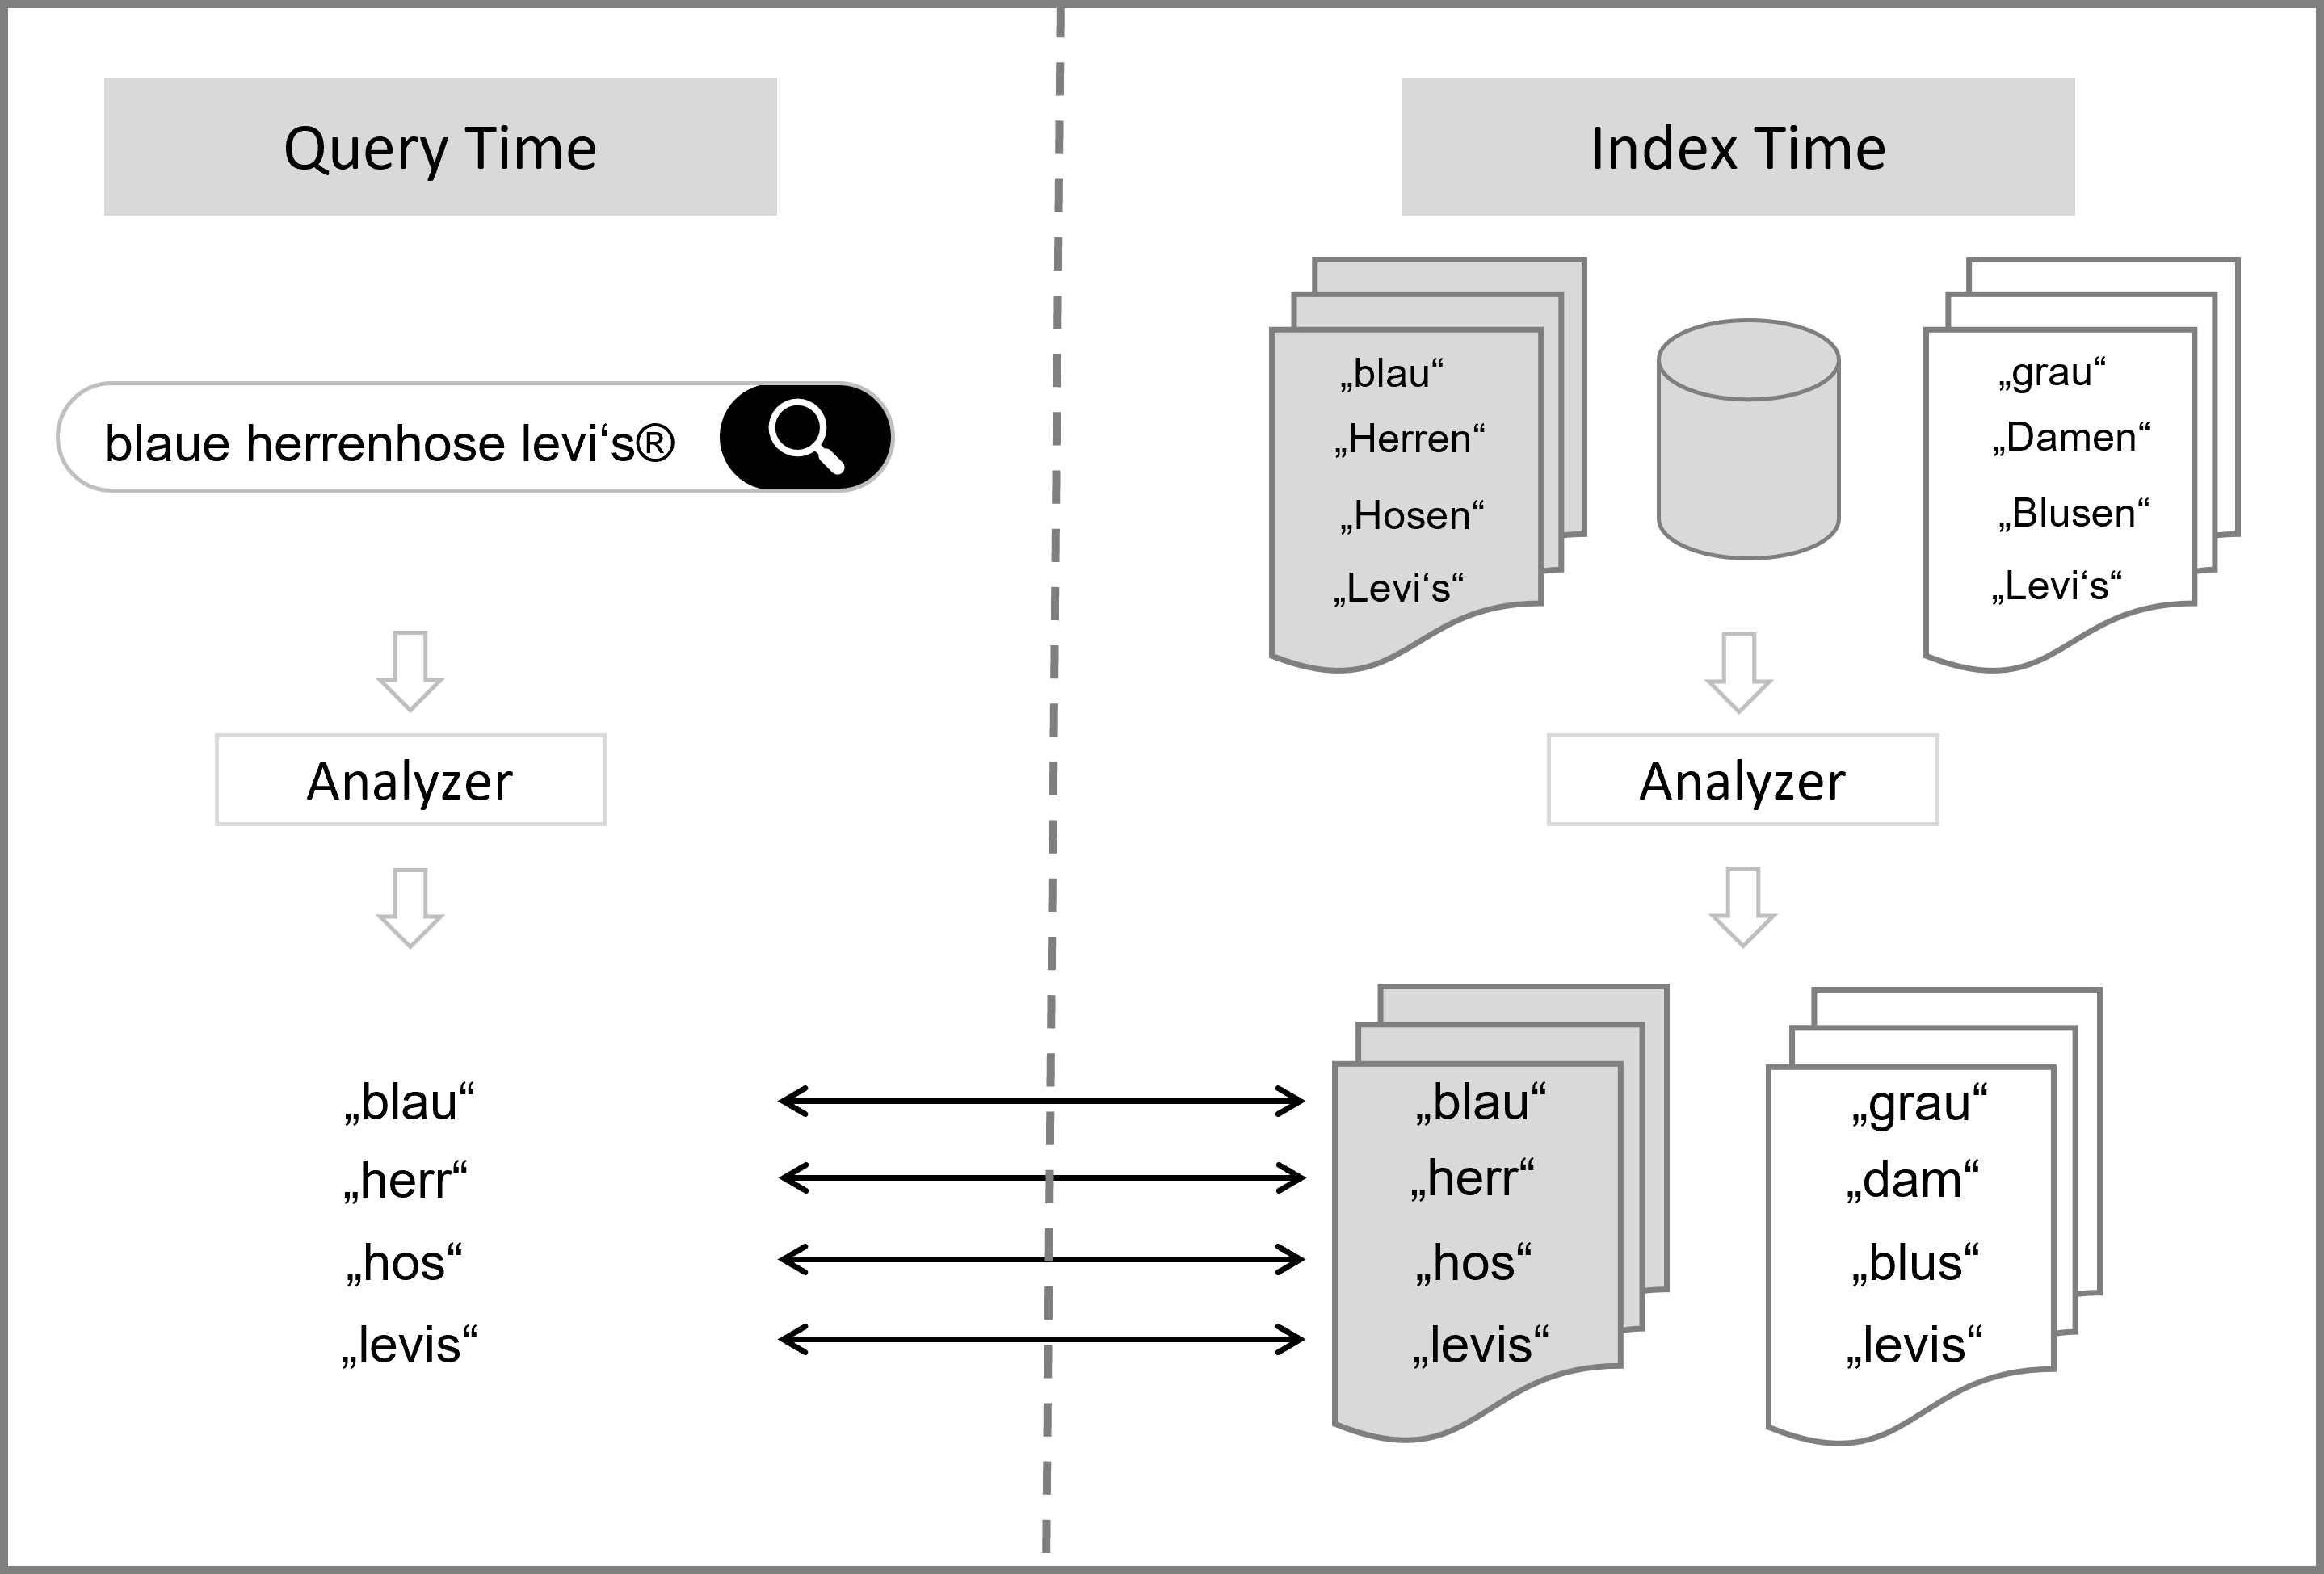
\includegraphics[width=0.7\linewidth]{images/Query_Index_Time.png}
    \caption{Analyzer bei Indexierung und Abfrage - in Anlehnung an \cite{SebastianRuss.2017}}
    \label{fig:final_index_ablauf}
\end{figure}

\subsection{Facettierte Suche\label{subsec2.1.3:Unterunterpunkt-3}}

Bei der Facetten-Suche wird die Menge der Suchergebnisse durch das Setzen von Filtern immer weiter eingeschränkt. Die Objekte und Produkte eines Informationssystems werden dabei mit Metadaten angereichert, welche die jeweiligen Facetten definieren. Der Begriff Facette beschreibt die verschiedenen Teilaspekte eines Objekts oder Produkts. So kann beispielhaft ein \glqq Hemd\grqq{} unteranderem mit den Facetten \glqq Größe\grqq{}, \glqq Farbe\grqq{} oder \glqq Muster\grqq{} versehen werden.

Eine Mindestanforderung nach Sperling \cite{Martin.2018} ist, dass die Filter sich dynamisch aus den bereits gefundenen Suchergebnistreffern bilden. So wechseln dynamisch die Filtermöglichkeiten je nach Suchergebnis und sinnfreie Filtermöglichkeiten beziehungsweise Filtermöglichkeiten ohne Suchergebnisse werden vermieden. In der Praxis ist ein solch dynamischer Wechsel der Filtermöglichkeiten in Online-Shops zu finden. Ein Benutzer ist zum Beispiel bei einem USB-Stick daran interessiert mithilfe eines Filters die maximale Datenmenge zu begrenzen und bei der Suche nach Waschmaschinen ist die Angabe des maximalen Fassungsvermögen eine aussagekräftige Filterung.

Wie in \autoref{fig:schubert_search} zu erkennen ist, kann man diese Filter mit unterschiedlichsten Bedienelementen visualisieren. Dabei ist zu unterscheiden, ob die Werte der Facetten explizit genannt werden können oder sich in einem Bereich befinden. Wie von Schubert Motors \cite{SchubertMotorsGmbH.2021} in \autoref{fig:schubert_search} umgesetzt, wurde zum Beispiel für die Preis-Facette ein Slider und für die Auswahl der Marke ein Drop-Down-Bedienelement ausgewählt.

\begin{figure}[H]
    \centering
    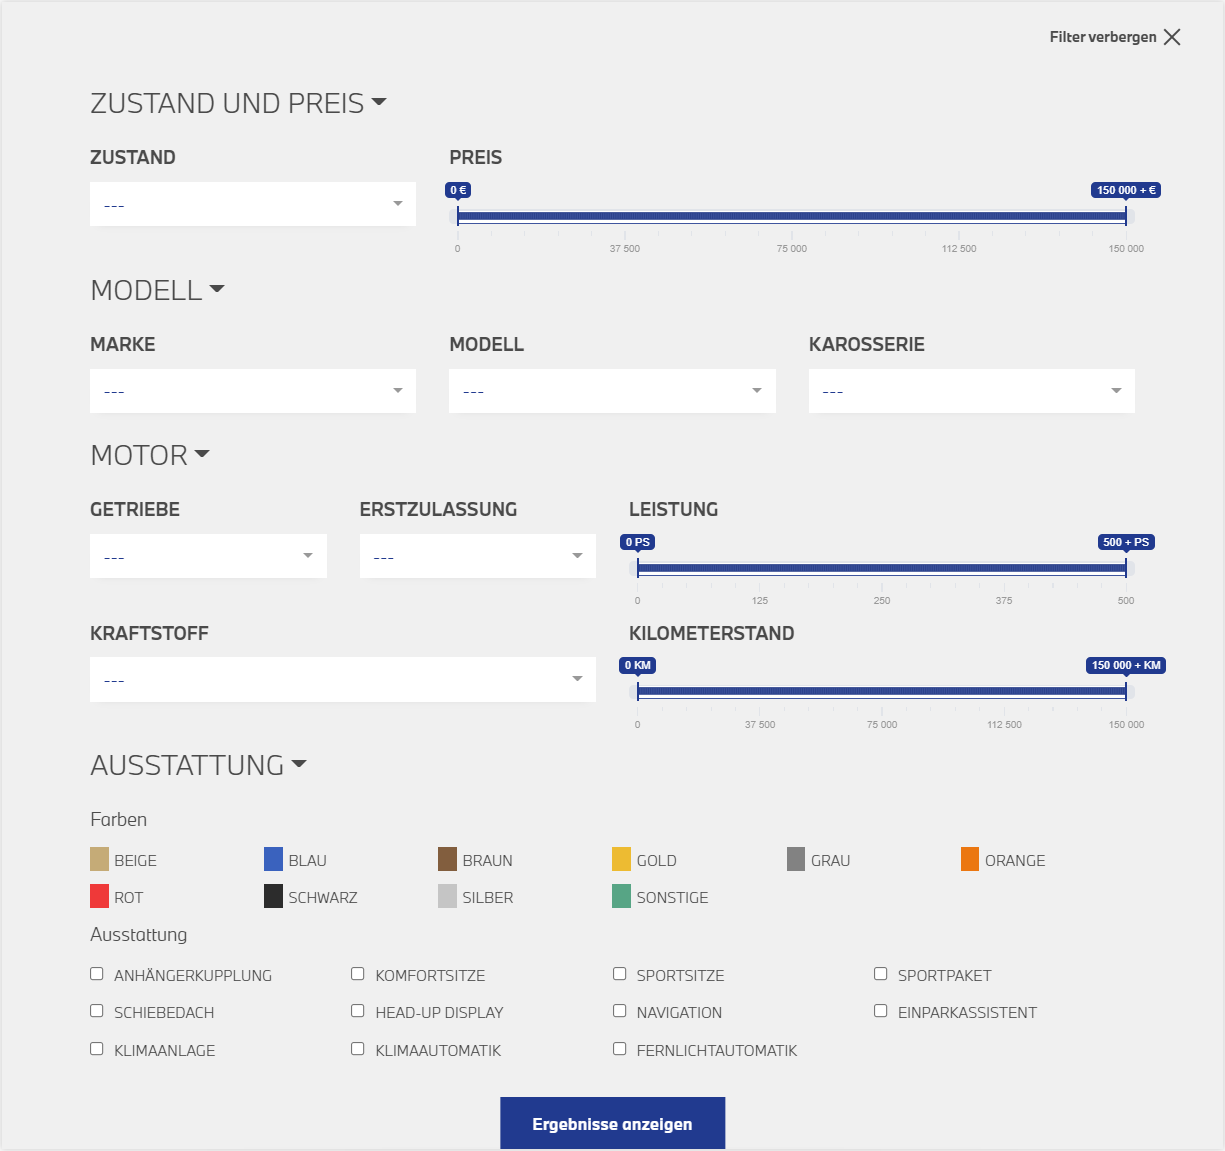
\includegraphics[width=0.85\linewidth]{images/schubert_search.png}
    \caption{Facettierte Suche bei Schubert Motors \cite{SchubertMotorsGmbH.2021}}
    \label{fig:schubert_search}
\end{figure}

Bei der praktischen Umsetzung einer facettierten Suche müssen die logischen Verknüpfungen zwischen den einzelnen Filter konfiguriert werden \cite{Martin.2018}. Aus den Ergebnissen der unterschiedlichen Filter müssen Vereinigungs- oder Schnittmengen gebildet werden, welche wiederum sortiert, durch eine Relevanzbestimmung, dem Benutzer präsentiert werden. Zum Einsatz kommen hierfür neben \glqq UND\grqq{}- auch \glqq ODER\grqq{}- Verknüpfungen. Die Wahl der richtigen Verknüpfung ist vom jeweiligen Kontext abhängig. So ist die Intention eines Benutzers bei der Benutzung der Facette \glqq Farbe\grqq{}, dass die einzelnen Ergebnisse mit einer ODER-Verknüpfungen miteinander kombiniert werden. Ein Benutzer erhält somit beispielsweise als Ergebnis alle Produkte der Farbe rot \textbf{UND} blau. Verwendet man jedoch mehrere Facetten bei der Suche, wie zum Beispiel die \glqq Farbe\grqq{} und \glqq Größe\grqq{}, ist die Schnittmenge aus den Ergebnissen von Vorteil. Hier ist eine UND-Verknüpfungen notwendig.

\subsection{Semantische Suche\label{subsec2.1.4:Unterunterpunkt-4}}

Während die Varianten \glqq Volltextsuche\grqq{} und \glqq Facettierte Suche\grqq{} lediglich auf einer syntaktischen und statistischen Auswertung von einzelnen Suchbegriffen basieren, greift eine semantische Suche zusätzlich noch auf ein semantisches Modell zurück \cite[S. 4f]{Hoppe.2020}. Solch ein, auch als \glqq Wissensmodell\grqq{} bezeichnetes, semantisches Modell, beschreibt die begrifflichen Zusammenhänge und Beziehungen. Dadurch ist es möglich neben syntaktisch ähnlichen, auch inhaltlich verwandte Treffer zu finden \cite[S. 3]{Hoppe.2020}. Nach Hoppe \cite[S. 3]{Hoppe.2020} kann demnach eine semantische Suche, im Sprachgebrauch der Künstlichen Intelligenz, als wissensbasiert bezeichnet werden.

Ziel ist es, die Suchfunktion weiter der menschlichen Sprache anzunähern. So liegt es, laut Tamblé \cite{MelanieTamble.2012}, in der Natur der menschlichen Sprache, dass mit verschiedenen Wörtern inhaltlich gleiche oder ähnliche Bedeutungen gemeint sind. So kann eine Landfläche in der deutschen Sprache auch mit den Begriffen \glqq Bereich\grqq{}, \glqq Gebiet\grqq{} oder \glqq Areal\grqq{} beschrieben werden. Neben Synonymen werden Begriffe auch durch Assoziationen miteinander verbunden. So wird der Begriff \glqq Rot\grqq{} mit dem Begriff \glqq Liebe\grqq{} assoziiert.

Für die Umsetzung einer semantischen Suche bedarf es einer Wissensdatenbank, in welcher Entitäten und deren Beziehungen untereinander abgespeichert werden. Mit dem Knowledge Graphen betreibt Google seit 2012 solch eine Wissensdatenbank, um Funktionen einer semantischen Suche bereitzustellen \cite{OlafKopp.2021}. Der Knowledge Graph wird dabei in drei Ebenen unterteilt: \cite{OlafKopp.2021}

\begin{description}
    \item[Entitäten-Katalog:]\hfill \\
    Die unterste Ebene ist eine reine Auflistung der verschiedenen Entitäten, welche über die Zeit hinweg identifiziert wurden. Die Art der Entitäten ist abhängig vom Kontext der Anwendung, in welcher eine Suchfunktion integriert ist. Allgemein handelt es sich um Objekte und Konzepte, welche eindeutig identifiziert werden können. Darunter zählen zum Beispiel Persönlichkeiten, Orte, Organisationen oder auch Farben und Gefühle.
    \item[Knowledge Repository:]\hfill \\
    Die unterschiedlichen Entitäten aus dem Entitäten-Katalog werden im Knowledge Repository mit Informationen beziehungsweise Attributen erweitert. Neben dem Ergänzen der Entitäten um Beschreibungen, werden diese auch in semantische Klassen und Gruppen eingeteilt. Die Gruppierungen werden auch Entitätstypen genannt.
    \item[Knowledge Graph:]\hfill \\
    Im eigentlichen Graphen werden die Beziehungen zwischen den unterschiedlichen Entitäten hergestellt.
\end{description}

In \autoref{fig:baby_yoda_google} ist das Ergebnis einer semantische Suchanfrage von Google abgebildet. Gesucht wurde mit der Suchphrase \glqq \textbf{small green guy with lightsaber as child}\grqq{}. Als Ergebnis erhält der Benutzer eine sofortige Übersicht über das wahrscheinlichste Ergebnis. In diesem Beispiel wurden die einzelnen Begriffe aus der Suchphrase mit dem Knowledge-Graphen von Google verglichen. Dabei erwiesen die Beziehungen der Begriffe untereinander, dass der fiktive Charakter \glqq Grogu\grqq{} am wahrscheinlichsten gesucht wird. 

Während bei einer reinen syntaktischen Suchfunktion die einzelnen Begriffe durch Transformationsschritte vereinheitlicht und anschließend mit einem invertierten Index verglichen werden, kann die semantische Suche nun auch mit Synonymen und Assoziationen umgehen. So würde die Suchmaschine Google das gleiche Ergebnis, wie in \autoref{fig:baby_yoda_google}, liefern, wenn statt dem Begriff \glqq small\grqq{} das Synonym \glqq little\grqq{} verwendet wird.

\begin{figure}[H]
    \centering
    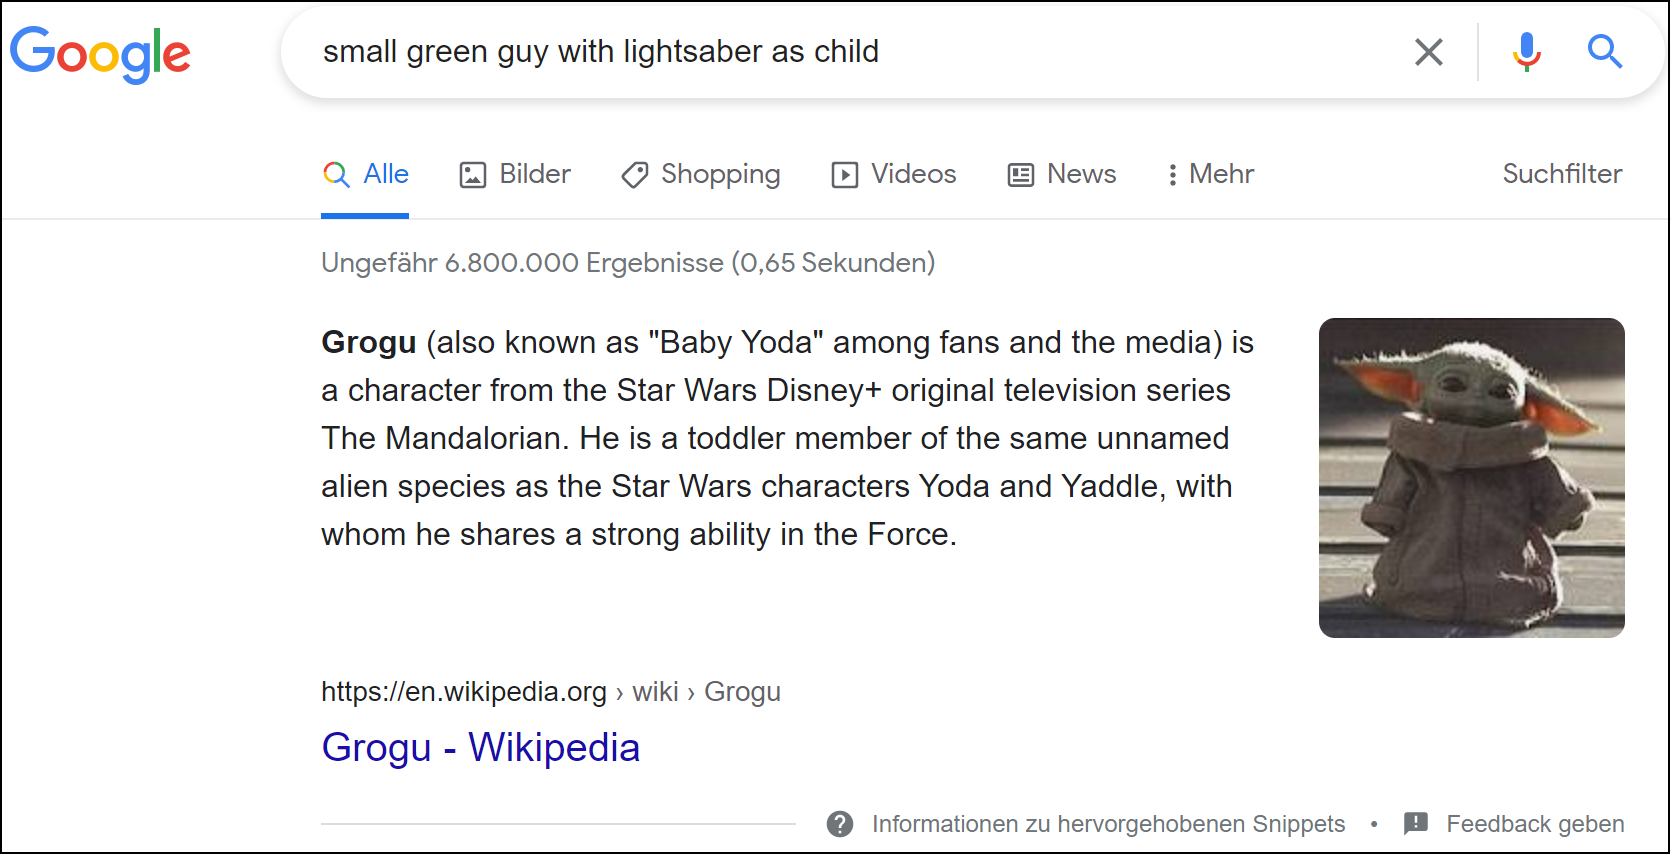
\includegraphics[width=1\linewidth]{images/baby_yoda.png}
    \caption{Ergebnis einer semantischen Suche in Google}
    \label{fig:baby_yoda_google}
\end{figure}

Um genauere und personalisierte Suchergebnisse zu erhalten, verwendet Google bei der semantischen Suche zusätzlich noch die persönlichen Daten und den Suchverlauf der Benutzer \cite{MichalPecanek.2020b}. So ist ein Programmierer mit der Suchphrase \glqq Python\grqq{} eher daran interessiert Suchergebnisse über die selbige Programmiersprache zu erhalten, anstatt über das Tier.

\subsection{Relevanzbestimmung\label{subsec2.1.5:Unterunterpunkt-5}}

Unabhängig, ob eine Volltextsuche, facettierte Suche, semantische Suche oder eine Kombination zum Einsatz kommt, müssen die Ergebnisse der Suchanfrage in einer geeigneten Reihenfolge angezeigt werden. Es gilt die einzelnen Treffer der Suche mit einer Relevanz zu gewichten und dem Benutzer die Treffer mit der höchsten Relevanz als erstes anzuzeigen.

Eine Möglichkeit der praktischen Umsetzung einer Relevanzbestimmung ist die Durchführung einer Termgewichtung mit dem \glqq TF-IDF\grqq{}-Modell. \glqq \gls{tf-idf}\grqq{} ist dabei ein statistisches Maß, welches angibt, wie relevant ein Begriff für ein Dokument in einer Sammlung von Dokumenten ist \cite{BrunoStecanella.2019}. Durch die Multiplikation der beiden Metriken \glqq \gls{tf}\grqq{} und \glqq \gls{idf}\grqq{} kann eine Sortierung der Suchergebnisse nach Relevanz erfolgen.

\subsubsection{Term Frequency - TF}

Eine der Metrik bezieht sich auf die Häufigkeit eines Begriffes in einem Dokument. Um diese Häufigkeit zu bestimmen, gibt es verschiedene Möglichkeiten. Das einfachste Vorgehen ist die reine Zählung des Vorkommens des Begriffes in einem Dokument \cite{BrunoStecanella.2019}. Weitergehend kann man die Häufigkeit auch nach der Länge des Dokumentes oder nach der Häufigkeit des häufigsten Wortes abhängig machen \cite{BrunoStecanella.2019}.

Unter der Einbeziehung der Gesamtzahl aller Terme eines Dokumentes, wird mit folgender Formel \cite{JensFrohlich.2020} die Begriffshäufigkeit eines Begriffes berechnet:

\begin{equation}
    \nonumber
    TF\textsubscript{(i)} = \frac{\log_2 (Freq(i,j) + 1)}{\log_2 (L)}
\end{equation}

\begin{itemize}
    \item i = Term
    \item j = Dokument
    \item L = Gesamtzahl aller Terme im Dokument j
    \item Freq(i,j) = Häufigkeit des Terms i im Dokument j
\end{itemize}

\subsubsection{Inverse Document Frequency - IDF}

Multipliziert wird die erste Metrik mit der inversen Dokumentenhäufigkeit. Darunter versteht man die Häufigkeit des Vorkommens eines Begriffes über die gesamte Dokumentenmenge hinweg. Einem Begriff wird hierbei ein größerer IDF-Wert zugeordnet, wenn der Begriff seltener vorkommt. Stopwords würden hierbei einen niedrigen IDF-Wert erhalten, da diese Begriffe in vielen Dokumenten vorkommen.

Für die Berechnung der invertierten Dokumentenhäufigkeit wird folgende Formel \cite{JensFrohlich.2020} verwendet: 

\begin{equation}
    \nonumber
    IDF\textsubscript{t} = \log (\frac{N\textsubscript{D}}{f\textsubscript{t}})
\end{equation}

\begin{itemize}
    \item t = Term
    \item N\textsubscript{D} = Gesamtzahl der Dokumente in der Dokumentensammlung D
    \item f\textsubscript{t} = Anzahl aller Dokumente, die t enthalten
\end{itemize}

Für die Bestimmung der Relevanz eines Begriffes in einem Dokument, wird die Multiplikation beider Metriken benötigt. Bei lediglich der Bestimmung der Begriffshäufigkeit, würden Stopwords eine große Relevanz bekommen. Erst durch die Einbeziehung der inversen Dokumentenhäufigkeit werden solche Begriffe, wie Stopwords mit einer niedrigeren Relevanz versehen.

\subsubsection{Beispiel}

Bei der Anwendung des TF-IDF - Wertes für die Relevanzbestimmung der Suchtreffer, werden die IDF-Werte der einzelnen Begriffe aus der Suchphrase miteinander verglichen. Sucht der Benutzer zum Beispiel nach der Suchphrase \glqq Website Analytics\grqq{}, wird vermutlich dem Begriff \glqq Website\grqq{} ein niedriger IDF-Wert zugeordnet, da dieser Begriff in vielen Dokumenten vorkommt.

Weitergehend werden dann die jeweiligen TF-Werte bestimmt. Hierbei wird jeder Begriff aus der Suchphrase mit jedem Dokument aus der Trefferliste in die TF-Formel eingegeben. So wird ein Dokument, welches den Begriff \glqq Analytics\grqq{} häufig enthält einen hohen TF-Wert erhalten.

Durch die Multiplikation beider Metriken pro Dokument kann eine Sortierung nach Relevanz durchgeführt werden.

\section{Software-Architekturen\label{sec2.2:Unterpunkt-2}}

\begin{quote}
    Die Software-Architektur eines Systems ist die Menge von Strukturen, die benötigt werden, um Entscheidungen über das System zu treffen, welche die Software-Elemente, die Relationen zwischen ihnen und die Eigenschaften von beiden betreffen. \textasciitilde{} Len Bass \cite[S. 4]{Bass.2013}
\end{quote}

Wie aus der Definition von Len Bass zu entnehmen ist, beschreibt eine Software-Architektur die Eigenschaften und Beziehungen von Software-Bausteinen zueinander \cite[S. 4]{Bass.2013}. Ein Software-Baustein wird hierbei als eine Teil-Komponente der gesamten Software betrachtet und wird bei der Erstellung einer Architektur als elementarer Bestandteil angesehen. Dabei wird ein Software-Baustein nicht näher spezifiziert, sondern als Komponente betrachtet, dessen konkrete Implementierung für die Architektur nicht von Bedeutung ist. Der Fokus einer Software-Architektur liegt auf den Schnittstellen der Software-Bausteine, über welche die Bausteine miteinander kommunizieren können.

\subsection{Architektur-Prinzipien\label{subsec2.2.1:Unterunterpunkt-1}}

Für das Erstellen einer guten Software-Architektur wurden von Vogel \cite[S. 128-147]{Vogel.2009} einige Grundprinzipien definiert. Diese Prinzipien sollten bei der Erstellung einer Software-Architektur beachtet werden: \cite[S. 128-147]{Vogel.2009}

\begin{description}
    \item[Lose Kopplung:]\hfill \\
    Der Kern einer Software-Architektur besteht aus der Beschreibung der Software-Bausteine eines Software-Systems und deren Interaktionen zueinander. Unter dem Begriff Kopplung versteht man hierbei die Beziehung unter den Software-Bausteinen einer Software-Architektur. Eine Kopplung charakterisiert demnach die Interaktionen der Software-Bausteine.

    Eine starke Kopplung von Software-Bausteinen hat zur Folge, dass beim Verstehen und Ändern eines Software-Bausteines auch zwingend weitere Software-Bausteine verstanden und geändert werden müssen. Um jenes Problem zu umgehen, besagt das Prinzip der losen Kopplung, dass die Kopplung zwischen Software-Bausteinen möglichst niedrig gehalten werden sollen.

    Um eine lose Kopplung in einer Architektur zu erreichen, ist die Einführung von Schnittstellenabstraktionen ein wichtiger Aspekt. Dabei werden die Implementierungsinformationen hinter den Schnittstellen verborgen. Durch die Begrenzung von Schnittstellenelementen und der Häufigkeit des Austauschs der Schnittstellenelemente, kann eine Kopplung von Software-Bausteinen kontrollierbar gemacht werden.

    \item[Hohe Kohäsion:]\hfill \\
    Im Gegensatz zur Kopplung, in welcher die Beziehungen zwischen Software-Bausteinen gemeint ist, versteht man unter dem Begriff Kohäsion die Abhängigkeiten innerhalb eines Software-Bausteins.

    Beim Prinzip der hohen Kohäsion ist das Ziel die Abhängigkeiten innerhalb eines Software-Bausteins möglichst hoch zu gestalten. Wie bei der losen Kopplung geht es auch hier um die lokale Änderbarkeit und Verstehbarkeit von Software-Bausteinen.
    
    Wie in \autoref{fig:kopplung_and_kohaesion} zu erkennen, stehen Kopplung und Kohäsion normalerweise miteinander in einer Wechselbeziehung. Hierbei gilt, dass je höher die Kohäsion individueller Software-Bausteine einer Architektur ist, desto geringer ist die Kopplung zwischen den Software-Bausteinen. Schematisch ist dieser Zusammenhang in \autoref{fig:kopplung_and_kohaesion} abgebildet, worin zu erkennen ist, das eine Gesamtstruktur mit einer hohen Kohäsion und einer losen Kopplung (rechte Seite) eine höhere Übersichtlichkeit besitzt.

    \begin{figure}[H]
        \centering
        \includegraphics[width=0.7\linewidth]{images/Kopplung_und_Kohäsion.png}
        \caption{Zusammenspiel von loser Kopplung und hoher Kohäsion - \cite{Vogel.2009}}
        \label{fig:kopplung_and_kohaesion}
    \end{figure}

    \item[Entwurf für Veränderung:]\hfill \\
    Durch den stetigen Wandel von Software-Systemen in Form von Anforderungen und Technologien, ist es von Vorteil solche Änderungen bereits in der Phase der architekturellen Konzeption zu berücksichtigen. Das Prinzip des Entwurfs für Veränderung (englisch: Design for Change) sieht nun vor, dass man vorhersehbare Änderungen architektonisch vorausplant. Dabei sollte man versuchen, die Architektur so zu entwerfen, dass man leicht mit den wahrscheinlichen Änderungen eines Software-Systems umgehen kann.

    \item[Separation of Concerns:]\hfill \\
    Abgeleitet von dem römischen Prinzip \glqq Teile und herrsche\grqq{} wird beim Prinzip Separation of Concerns ausgesagt, dass ein Software-System in individuelle Software-Bausteine zerlegt werden soll.

    Separation of Concerns unterstützt hierbei die Modularisierung eines Software-Systems. Es geht darum Teile eines Software-Systems zu identifizieren, welche für bestimmte Angelegenheiten, Aspekte und Aufgaben verantwortlich sind. Jene Teile werden dann als eigene Software-Bausteine gekapselt. Eine Zerteilung des Gesamtsystems in relativ unabhängige Einzelteile ermöglicht zudem noch die Verteilung von Verantwortlichkeiten für verschiedene Software-Bausteine und auch das parallele Arbeiten an dem Software-System durch mehrere Entwickler wird dadurch ermöglicht.

    Durch das Aufteilen des Software-Systems in relativ unabhängige Software-Bausteine, werden auch die Prinzipien lose Kopplung und hohe Kohäsion begünstigt.

    \item[Information Hiding:]\hfill \\
    Das Prinzip Information Hiding sagt aus, dass man einem Klienten nur die für die Bearbeitung eines Problems notwendigen Informationen zeigen soll. Dies erleichtert die Gliederung und das Verständnis von komplexen Software-Systemen. Die restlichen Informationen sollen nach außen hin verborgen bleiben. Ermöglicht wird solch ein \glqq geheim halten\grqq{} von Informationen durch die Bereitstellung von definierten Schnittstellen, über welche nur bestimmte Informationen zu erreichen sind.

    \item[Abstraktion:]\hfill \\
    Als übergeordnetes Prinzip dient eine Abstraktion dazu, ein komplexes System verständlicher zu machen. Dazu werden wichtige Aspekte identifiziert und unwichtige Details vernachlässigt. Im Bereich der Software-Architektur gilt die Schnittstellenabstraktion als Teilprinzip der Abstraktion. Hierbei liegen die Schnittstellen im Fokus, welche für das Zustandekommen und die Qualität von Beziehungen verantwortlich sind.

    Solch eine Schnittstellenabstraktion in einem Software-System ist eng verbunden mit dem Prinzip der losen Kopplung und dem Information Hiding. Ein Aspekt für den starken Zusammenhang zwischen der Abstraktion und dem Information Hiding ist die Portabilität von Software-Systemen. So sollte eine Architektur oder ihre Software-Bausteine auch in anderen Umgebungen verwendbar sein. Um solch eine Plattformunabhängigkeit sicherzustellen, werden Abstraktionen verwendet, die ein Information Hiding der Platform-Details leisten.

    \item[Modularität:]\hfill \\
    Das Modularitätsprinzip, welches bereits auch in den Beschreibungen der anderen Prinzipien vorkam, definiert die Aufteilung eines Systems in klar definierte Software-Bausteine mit abgegrenzten funktionalen Verantwortlichkeiten. Die Modularität ist dabei eine Kombination aus den Prinzipien Abstraktion, Separation of Concerns und Information Hiding, welche bei der Umsetzung der Prinzipien der losen Kopplung und der hohen Kohäsion kombiniert werden.

\end{description}

Auch für die spätere Konzeption einer Volltextsuche in einer Microservice-Architektur werden die eingeführten Prinzipien als Grundlage dienen.

\subsection{Monolithische und verteilte Architekturen\label{subsec2.2.2:Unterunterpunkt-2}}

Bei der Neugestaltung von E-MES wird von einer monolithischen 3-Schichten-Architektur auf eine verteilte Microservice-Architektur gewechselt.

In einer monolithischen Architektur wird die gesamte Architektur in nur einem Software-Baustein zusammengefasst. Dadurch erfolgt keine explizite Gliederung in Teilsysteme und Architektur-Prinzipien, wie lose Kopplung und Separation of Concerns sind nur schwer umsetzbar \cite[S. 216]{Vogel.2009}. Zu finden sind monolithische Architekturen oftmals in Altsystemen, welche oft über Jahrzehnte gewachsen sind. Aufgrund der mangelnden Modularisierung steigt die Komplexität des Systems. Die Wartung und Anpassung des Quellcodes wird erschwert \cite{Prof.Dr.AndreasFink.2012b}. Ein weiterer Nachteil der mangelnden Modularisierung ist die kaum mögliche nebenläufige Ausführung von Teilen des Systems auf verschiedenen Rechnern \cite{Prof.Dr.AndreasFink.2012b}. Somit kann eine horizontale Skalierung nicht ermöglicht werden, und eine effiziente, lastverteilende Programmausführung ist nicht gegeben.

Die Architektur von MCC wird eine verteilte Struktur aufweisen. Hierbei werden Teile des Gesamtsystems in unterschiedliche Software-Bausteine aufgeteilt. Eine Modularisierung der Software ist dadurch möglich und Architekturen-Prinzipien, wie lose Kopplung und Separation of Concerns sind umsetzbar \cite{Vogel.2009}. Durch die strikte Aufteilung der Geschäftslogik kann auch die Komplexität aufgeteilt werden. Somit können die einzelnen Software-Bausteine mit wenig Aufwand angepasst oder erweitert werden. Durch die Modularisierung von verteilten Architekturen kann die Ausführung bestimmter Aufgaben auf redundanter Hardware nebenläufig erfolgen \cite{Prof.Dr.AndreasFink.2012}. Durch jene horizontale Skalierung kann eine effiziente und lastverteilende Programmausführung erfolgen, welche auch zur Ausfallsicherheit des Gesamtsystems beiträgt \cite{Prof.Dr.AndreasFink.2012}.

\section{Microservice-Architektur\label{sec2.3:Unterpunkt-3}}

Bei der Neugestaltung des \gls{mes} der Firma Enisco wird auf eine Microservice-Architektur aufgebaut, welche eine verteilte Struktur aufweist.

Die Kernelemente dieser Architektur sind die Microservices, welche der Modularisierung der Software dienen. Der Begriff Microservice wird hierbei für kleine unabhängige Services verwendet, welche über klar definierte APIs miteinander kommunizieren \cite{AmazonWebServicesInc..2021}. Durch die lose Kopplung ist eine einfache Skalierbarkeit und unabhängige Entwicklung durch verschiedene Teams möglich. Dies wiederum verringert die Entwicklungszeit und Komplexität bei Wartung.

Durch die Verwendung von Microservices ist eine Aufteilung des Gesamtsystems in verschiedene Software-Bausteine möglich. Ein Software-Baustein stellt dabei jeweils eine Funktionalität des Gesamtsystems dar. Im Gegensatz zu einer monolithischen Architektur läuft das Gesamtsystem nicht innerhalb eines Prozesses, sondern auf verschiedenen Prozessen. Dabei wird jedem Software-Baustein ein eigener Prozess zugeordnet. Jene Prozesse können nun nahezu beliebig auf verschiedene Rechner verteilt und durch Replizierung ausfallsicher gemacht werden. \cite{GaryCalcott.2018}

Neben den Vorteilen der horizontalen Skalierung ergeben sich aus der Aufteilung des Gesamtsystems in unterschiedliche Software-Bausteine auch Auswirkungen auf die Entwicklungsorganisation. So wird beim Umgang mit Microservices nach der Unix-Philosophie von Ken Thompson \glqq Do one thing and do it well\grqq{} \cite{IONOSSE.2021} gearbeitet. Durch die Modularität von Microservices können diese von unterschiedlichen Entwicklerteams unabhängig entwickelt werden. Durch die Abstraktion der Microservices können diese mit unterschiedlichen Technologien und Programmiersprachen implementiert werden. Auch der Datenhaushalt kann von jedem Microservice separat verwaltet werden. Zudem wird die Einarbeitung eines Entwicklers in die Codebasis reduziert, da durch die Aufteilung weniger Code verstanden werden muss.

Die Microservice-Architektur berücksichtigt die Architektur-Prinzipien Separation of Concerns, Information Hiding und Modularität und gewährleistet somit eine lose Kopplung zwischen den Microservices. Innerhalb der Microservices entsteht dadurch eine hohe Kohäsion.

Da die jeweiligen Microservices repliziert auf verschiedenen Rechnern laufen können, ist die Kommunikation zwischen den Microservices schwieriger als bei einem monolithischen System. Auf die Kommunikation zwischen Microservices wird in \autoref{subsec2.2.1:Unterunterpunkt-1} näher eingegangen.

Eine Herausforderung bei der Konzeption einer Microservice-Architektur ist die Vermeidung von Abhängigkeiten, welche eine lose Kopplung der Microservices verhindern würden. Um solche monolithischen Seiteneffekte zu vermeiden, werden in \autoref{subsec2.2.2:Unterunterpunkt-2} die häufigsten Microservice-Anti-Pattern aufgezeigt.

\subsection{Kommunikation zwischen Microservices\label{subsec2.3.1:Unterunterpunkt-1}}

Auch wenn das Ziel einer Microservice-Architektur ist, dass einzelne Funktionalitäten des Gesamtsystems in getrennte Microservices gekapselt werden, müssen diese miteinander kommunizieren. Aufgrund der Modularität können die Microservices horizontal skaliert und auf verschiedenen Rechnern betrieben werden. Dies erhöht die Komplexität bei der Kommunikation der Microservices untereinander. \cite{MichaelSchwab.2019}

Bei der Wahl der Kommunikation zwischen Microservices kann zwischen einer synchronen und asynchronen Kommunikation entschieden werden.

\subsubsection*{Synchrone Kommunikation}

Bei der synchronen Kommunikation handelt es sich um eine eins-zu-eins Kommunikation, bei der eine Anfrage geschickt und auf eine Antwort gewartet wird. Klassischerweise erfolgt die Kommunikation über HTTP mit einer REST-Schnittstelle. \gls{rest} ist hierbei eine Spezifikation, wie eine über HTTP kommunizierende API konzipiert werden soll \cite{MichaelSchwab.2019}. Eine solche API sollte demnach vordefinierte HTTP-Methoden implementiert haben. Unter anderem sind das Methoden wie GET, POST, PUT und DELETE. Bei einer GET-Anfrage werden hierbei Ressourcen angefragt. Soll ein neuer Datensatz übermittelt werden, wird die POST-Methode verwendet. Zur Änderung eines bestehenden Datensatzes gibt es die PUT-Methode und mit der DELETE-Methode kann ein Datensatz entfernt werden. Jeder Datensatz bekommt hierbei einen eigenen Endpunkt, und die jeweiligen Anfragen können mit URL-Parametern und Query-Parametern spezifiziert werden. Das Standard-Datenformat bei REST ist JSON.

\label{service_discovery}Bei der Kommunikation von zwei Microservices über die jeweiligen REST-Schnittstellen muss die Adresse des anderen Microservice bekannt sein. Durch die Verteilung der Microservices auf unterschiedliche Rechner in Folge einer horizontalen Skalierung kann es während des Betriebes vorkommen, dass einzelne Microservices auf zum Beispiel Rechner A gestoppt und auf Rechner B wieder gestartet werden. Dadurch ändern sich auch die Adressen der Microservices. Da die Verwaltung der Adressen ab einer Vielzahl an Microservices nicht mehr trivial ist, wird in einer Microservice-Architektur eine sogenannte Service-Discovery eingesetzt. Die Service-Discovery ist eine Software, bei der sich alle neuen Microservices registrieren. Bei einem REST-Aufruf wird dann zuerst eine Liste mit allen verfügbaren Adressen abgerufen.

Wie in \autoref{fig:service_discovery} dargestellt ist, wird bei einer Anfrage eines Services, jene Anfrage zunächst an einen Router-Service geleitet. Nach dem Abfragen der Adresse mithilfe der Service-Discovery wird gezielt der entsprechende Service beziehungsweise dessen Instanz mit einer REST-Anfrage angesprochen.

\begin{figure}[H]
    \centering
    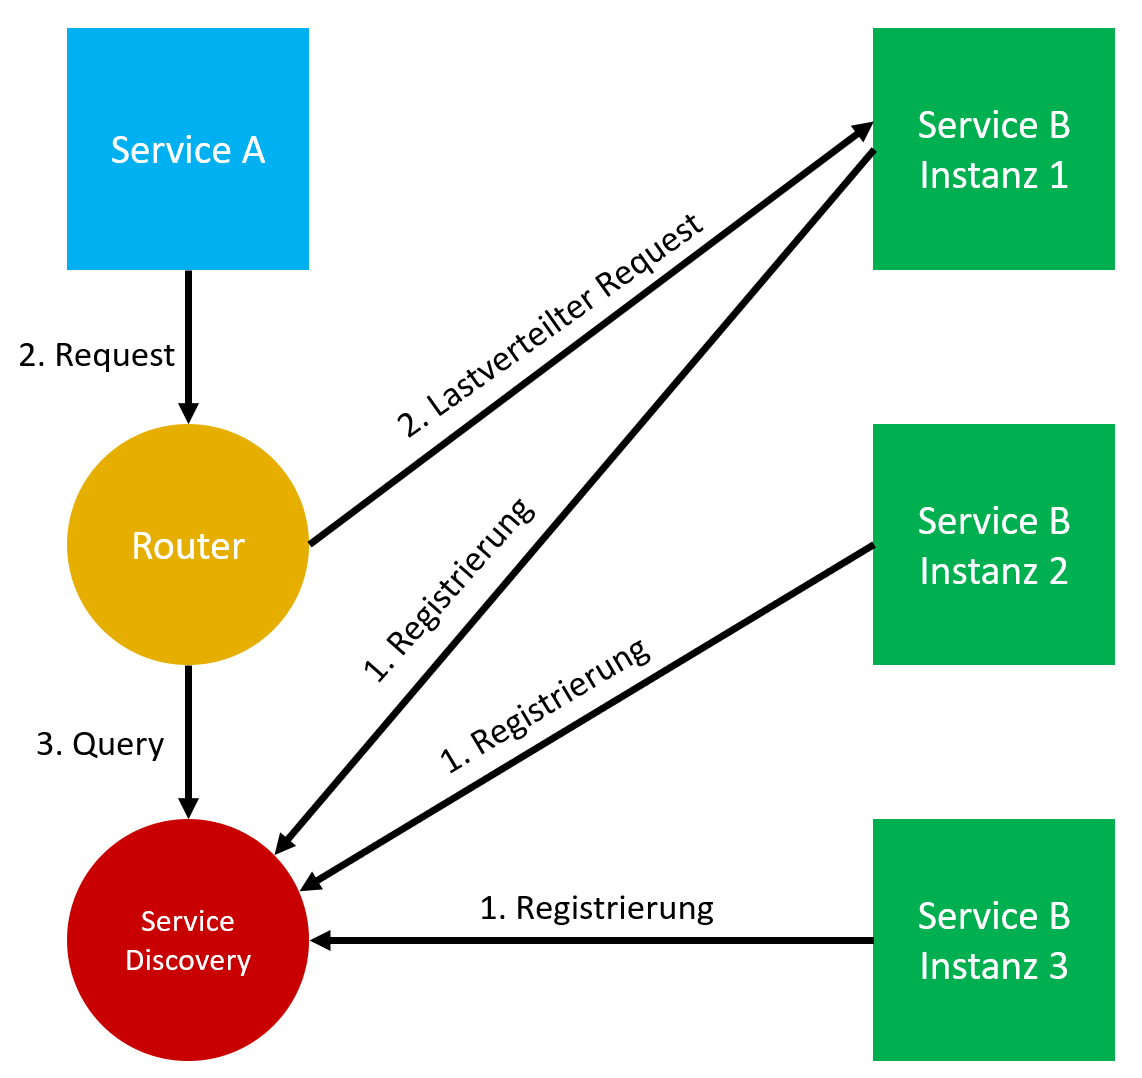
\includegraphics[width=0.65\linewidth]{images/service-discovery.png}
    \caption{Ablauf einer Anfrage mit der Service-Discovery - in Anlehnung an \cite{MichaelSchwab.2019}}
    \label{fig:service_discovery}
\end{figure}

\subsubsection*{Asynchrone Kommunikation}

Anders als bei der synchronen Kommunikation wird bei der asynchronen Kommunikation nicht auf jede Anfrage eine Antwort erwartet. Kern einer asynchronen Kommunikation ist ein zentraler Nachrichtenkanal, auf dem Nachrichten ausgetauscht werden. Ein Service schickt Nachrichten an solch einen Nachrichtenkanal, auch Message Broker genannt, und wenn ein anderer Service an der Nachricht interessiert ist, kann er diese konsumieren. Eine Nachricht kann dabei auch von mehreren Services konsumiert werden.

% Zu den bekanntesten Message Brokern zählen RabbitMQ und Apache Kafka. Während RabbitMQ leichtgewichtiger ist als Apache Kafka, hat letzteres mehr Features und weist eine größere Stabilität auf.

Die Verantwortlichkeiten innerhalb des Systems werden bei der Verwendung eines Message Brokers umgedreht. Ein Service wird nun nicht mehr explizit von einem anderen Service aufgerufen, sondern schickt seine Nachrichten an den Message Broker, ohne zu wissen, wer diese Nachrichten konsumiert. Sender und Empfänger sind somit lose gekoppelt.

Zur Einteilung der Nachrichten werden in Message Brokern sogenannte Message Queues verwendet. Über eine Message Queue, welche einen bestimmten Topic besitzt, können Services dann entweder Nachrichten senden oder sich als Konsumenten an diesem Topic registrieren. In \autoref{fig:Message_Broker_Queue} ist die Funktionsweise beispielhaft an dem Message Broker \glqq Apache Kafka\grqq{} abgebildet. Durch den Publish/Subscribe-Mechanismus kann Service A in diesem Beispiel sowohl Publisher von zwei Topics sein, als auch Konsument von einem Topic.

\begin{figure}[H]
    \centering
    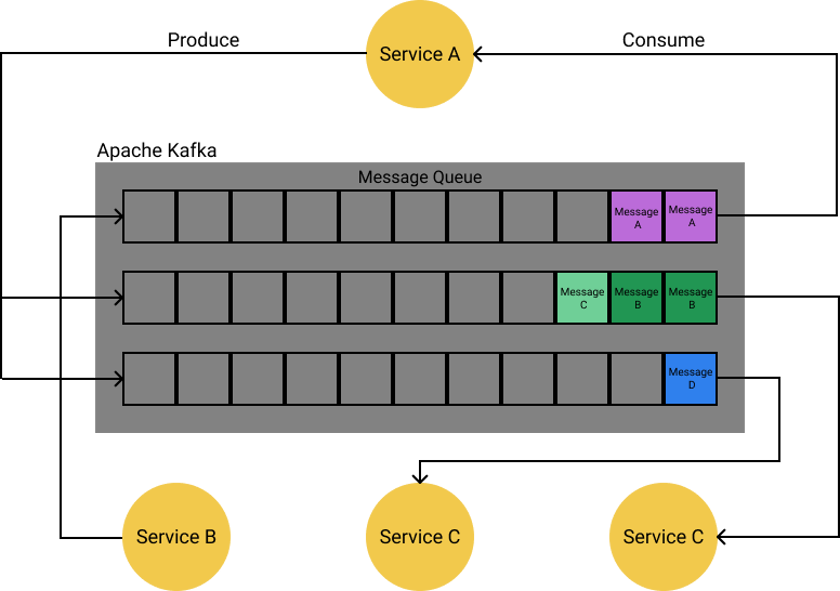
\includegraphics[width=0.65\linewidth]{images/apache-kafka.png}
    \caption{Funktion eines Message Brokers - \cite{MichaelSchwab.2019}}
    \label{fig:Message_Broker_Queue}
\end{figure}

Die Nachrichten werden in der Message Queue zwischengespeichert, bis die registrierten Konsumenten diese Nachrichten gelesen haben. Wenn ein Service sich an einer Message Queue registriert, können verschiedene Servicequalitäten für die Übertragung der Nachrichten angegeben werden. Folgende drei \glqq \gls{qos}\grqq{} können angegeben werden: \cite{ApacheSoftwareFoundation.2021}

\begin{description}
    \item[QoS 0 \glqq At most once\grqq{}:]\hfill \\
    Eine Nachricht wird genau einmal versendet. Nach dem Prinzip \glqq fire and forget\grqq{} wird keine Rückbestätigung erwartet. Verwendet wird diese Servicequalität meist für Nachrichten, welche mit einer hohen Frequenz versendet werden. So ist es für viele Sensoren in einer IoT-Umgebung nicht erforderlich, dass jeder gemessene Wert erfolgreich übermittelt wird.
    
    \item[QoS 1 \glqq At least once\grqq{}:]\hfill \\
    Es wird sichergestellt, dass eine Nachricht genau einmal beim Empfänger ankommt. Hierzu werden die Nachrichten beim Sender solange zwischengespeichert, bis vom Empfänger eine Bestätigung (PUBACK) empfangen wird. Wird über eine gewisse Zeitspanne keine Bestätigung empfangen, wird die Nachricht erneut versendet. Hierbei kann es vorkommen, dass ein Empfänger eine Nachricht mehrfach erhält. \cite{FlorianRaschbichler.2017}
    
    \item[QoS 2 \glqq Exactly once\grqq{}:]\hfill \\
    Eine Nachricht wird genau einmal zugesendet. Hierbei wird ein 4-Wege-Handshake zwischen Sender und Empfänger versendet. Durch diesen Ablauf ist eine sichere Übertragung der Nachricht gewährleistet. Durch den großen Overhead ist jedoch diese Servicequalität die langsamste Übertragungsmöglichkeit.

\end{description}

\subsection{Microservice - Anti-Pattern\label{subsec2.3.2:Unterunterpunkt-2}}

Um die Vorteile einer Microservice-Architektur im Bezug auf lose Kopplung und der damit eingehenden Unabhängigkeit der Microservices bezüglich Wartbarkeit und Erweiterbarkeit zu gewährleisten, ist es von Nöten die möglichen Anti-Pattern einer Microservice-Architektur zu kennen. Mit Hilfe von Anti-Pattern können nach Roth und Hafner \cite{StephanRoth.2019} wiederkehrende Fehler bei der Softwareentwicklung identifiziert und in generalisierter Form dokumentiert werden. So können Anti-Pattern dabei helfen häufig auftretende Fehler von vornherein zu vermeiden.

In einer Studie von Tighilt et al. \cite{Tighilt.072020} wurden 27 Paper und 67 Open-Source Anwendungen, welche alle Bezug zur Microservice-Architektur haben, untersucht. Die Ergebnisse der Studie \cite{Tighilt.072020} ergeben eine Sammlung von häufig aufgetretenen Anti-Pattern, welche durch Tighilt et al. in vier Kategorien unterteilt wurden. Folgend werden die Kategorien mit Beispielen erläutert:

\subsubsection*{Design Anti-Pattern}

In diese Kategorie gehören Anti-Pattern, welche bereits in der architektonischen Entwurfsphase einer Microservice-Architektur zu Fehlern führen. Beispiele sind hierfür das \glqq Falscher Schnitt\grqq{} - Anti-Pattern und das \glqq Zyklische Abhängigkeiten\grqq{} - Anti-Pattern.

\begin{description}
    \item[Falscher Schnitt:]\hfill \\
    Beim \glqq Falscher Schnitt\grqq{} - Anti-Pattern wird die Aufteilung des Gesamtsystems in unterschiedliche Microservices nicht nach Geschäftsfunktionen, sondern nach technischen Aspekten durchgeführt. Ähnlich wie bei einer monolithischen 3-Schichten-Architektur übernehmen dann ein Teil der Microservices die Präsentationsschicht, andere Microservices wiederum bedienen die Geschäftsschicht und die anderen bedienen die Datenzugriffsschicht. Durch dieses Vorgehen verliert die Architektur die lose Kopplung zwischen den Microservices, und die Modularität geht verloren. Auch müssen bei einer Änderung einer Geschäftslogik mehrere Microservice abgeändert werden, was zu einem Mehraufwand führt.

    Verhindert werden kann dieses Anti-Pattern, indem man die Trennung des Gesamtsystems anhand der Geschäftsfunktionen durchführt. Jeder Microservice sollte von einem Team implementiert und gewartet werden können. Die Abhängigkeiten zu anderen Microservices sollten so gering wie möglich ausfallen, um eine lose Kopplung und die Modularität der Architektur zu gewährleisten.
    
    \item[Zyklische Abhängigkeiten:]\hfill \\
    Ein weiterer Fehler ist die Missachtung der losen Kopplung, indem man mit zyklischen Abhängigkeiten eine starke Gebundenheit an andere Microservices verursacht. Dadurch müssen die abhängigen Microservices sowohl bei der Implementierung als auch bei der Wartung berücksichtigt werden. Dies erhöht die Komplexität und die Wahrscheinlichkeit, dass Fehler auftreten.

    Eine zyklische Abhängigkeit zwischen solchen Microservices kann verhindert werden, indem man stark voneinander abhängige Microservices in einen gemeinsamen Microservice zusammenfasst. 

\end{description}

\subsubsection*{Implementation Anti-Pattern}

% Implementation Anti-Pattern entstehen aus der Art und Weise wie Microservices implementiert werden. Beispiele sind hierfür das \glqq Gemeinsame Bibliotheken\grqq{} - Anti-Pattern und das \glqq Festcodierte Endpunkte\grqq{} - Anti-Pattern.

Implementation Anti-Pattern entstehen aus der Art und Weise wie Microservices implementiert werden. Beispiele sind hierfür das \glqq Festcodierte Endpunkte\grqq{} - Anti-Pattern.

\begin{description}
    % \item[Gemeinsame Bibliotheken:]\hfill \\
    % Bei der Verwendung von Bibliotheken in einer Microservice-Umgebung gilt es zwischen den Prinzipien \glqq \gls{dry}\grqq{} und \glqq Lose Kopplung\grqq{} abzuwägen.

    % Durch die gemeinsame Nutzung von Services, wird eine mehrfache Implementierung vermieden. Die Services werden dadurch aber stärker aneinander gekoppelt.

    % Werden einzelne Bibliotheken von mehreren Services verwendet, vermeidet man eine mehrfache Implementierung. 

    % Bei der Verwendung von gemeinsam genutzten Bibliotheken entstehen starke Abhängigkeiten, und die Bibliotheken stellen einen sogenannten \glqq Single point of failure\grqq{} dar.

    % Um dieses Problem zu umgehen, kann jedem Microservice seine eigene Bibliothek zur Verfügung gestellt werden. Dieser Ansatz wiederum führt zu einer Komplexität bei der Wartbarkeit der Microservice.
    
    % Ein weiterer Ansatz wäre es, die Bibliotheken durch einen Bibliothek-Service zu abstrahieren. Die Microservices bleiben lose gekoppelt und die Komplexität bei der Wartung bleibt überschaubar.
    
    \item[Festcodierte Endpunkte:]\hfill \\
    Bei der synchronen Kommunikation zwischen Microservices werden in der Regel Anfragen über REST APIs gestellt. Hierfür müssen die IP-Adresse und der Port des anderen Microservices bekannt sein. Ein Ansatz für schnelle Laufzeiten und eine einfache Implementierung ist es, die Endpunkte fest im Quellcode zu hinterlegen. Dieser Ansatz ist jedoch bei einer größeren Anzahl von Microservices nicht mehr wartbar. Sobald sich ein Endpunkt eines Microservice ändert, müssen alle abhängigen Microservices geändert und neu deployed werden.

    Abhilfe bringt die Einführung einer Service-Discovery (Siehe auch \autoref{service_discovery}), bei welcher sich die einzelnen Services registrieren. Ein anfragender Service kann nun über diese Service-Discovery die aktuelle Adresse des anderen Services erhalten.

\end{description}

\subsubsection*{Deployment Anti-Pattern}

Auch in der Bereitstellungsphase einer Microservice-Architektur können Fehler auftreten. Diese Anti-Pattern werden Deployment Anti-Pattern genannt. Beispiele sind hierfür das \glqq Manuelle Konfiguration\grqq{} - Anti-Pattern und das \glqq Zeitüberschreitungen\grqq{} - Anti-Pattern.

\begin{description}
    \item[Manuelle Konfiguration:]\hfill \\
    In einer Microservice-Architektur müssen aufgrund der Verteilung der Microservices auf unterschiedliche Rechner verschiedene Konfigurationen durchgeführt werden. Eine manuelle Konfiguration von jedem Microservice führt zu unzähligen Konfigurationsdateien und Abhängigkeiten zu Umgebungsvariablen. Mit wachsender Anzahl von Microservices führt die manuelle Konfiguration zu einer ansteigenden Komplexität bei der Wartung der Konfigurationen.

    Durch die Einführung eines Konfigurations-Servers kann dieses Anti-Pattern vermieden werden. Durch geeignete Konfigurationsmanagement-Tools können sämtliche Konfigurationen zentral verwaltet werden.
    
    \item[Zeitüberschreitungen:]\hfill \\
    In einer verteilten Microservice-Architektur kann es vorkommen, dass einzelne Services ausfallen und nicht mehr zur Verfügung stehen. Hat nun ein anderer Microservice eine Anfrage über eine REST API gestellt, kann es vorkommen, dass unter Umständen gar keine Antwort kommt. Hierfür kann der Entwickler Timeouts festlegen, nach welchen einem anfragenden Service mitgeteilt wird, dass ein anderer Service nicht erreichbar ist. Den richtigen Wert für solch einen Timeout zu wählen, hängt von der Art des Service ab. Ein zu kurzer Timeout kann dazu führen, dass langsame Service frühzeitig beendet werden. Bei einer zu langen Wahl des Timeouts kann es vorkommen, dass der Endnutzer zu lange warten muss, bis ihm signalisiert wird, dass der gewünschte Service nicht verfügbar ist.

    Um dem entgegen zu wirken, verwendet man in einer Microservice-Architektur üblicherweise einen Circuit Breaker. Ein Circuit Breaker überwacht hierbei alle Instanzen einzelner Microservices und stellt fest, ob einzelne Timeouts bei der Kommunikation mit der jeweiligen Instanz überschritten wurden. Da solch ein Circuit Breaker als Proxy für alle Kommunikationskanäle verwendet wird, werden alle Anfragen an einen ausgefallenen Service mit einer Fehlermeldung beantwortet. Die Anfragen werden solange durch den Circuit Breaker blockiert, bis der ausgefallene Service wieder zur Verfügung steht. Auch der Timeout des Circuit Breaker muss vom Entwickler festgelegt werden.

\end{description}

\subsubsection*{Monitoring Anti-Pattern}

Zu dem Betrieb einer Microservice-Architektur gehört auch die Überwachung der Änderungen im System. Hierbei kann es auch zu häufig auftretenden Anti-Pattern kommen. Beispiele sind hierfür das \glqq Kein Gesundheitscheck\grqq{} - Anti-Pattern und das \glqq Lokale Protokollierung\grqq{} - Anti-Pattern.

\begin{description}
    \item[Kein Gesundheitscheck:]\hfill \\
    In der Natur der Microservices kann es vorkommen, dass einige Services über gewisse Zeitspannen nicht erreichbar sind. Um ein kompletten Systemausfall zu vermeiden, dienen Mechanismen, wie der Circuit Breaker, dazu die anfragenden Services über das Überschreiten von Timeouts zu benachrichtigen.

    Mit der Integration von Gesundheitschecks können solche Ausfälle von einzelnen Services im Voraus erkannt und abhängige Microservices darüber informiert werden, dass das Senden von Anfragen zu unterlassen ist. Für solche Gesundheitschecks werden API-Endpoints angeboten, welche periodisch abgefragt werden können.
    
    \item[Lokale Protokollierung:]\hfill \\
    Um eine spätere Fehlerdiagnose zu ermöglichen, speichern Microservices einige Informationen über Änderungen in Log-Dateien. Ein häufiger Fehler ist, dass solch eine Protokollierung lokal in den Datenbanken der einzelnen Microservices gespeichert werden. Die Herausforderung liegt nun bei der Analyse und Abfrage von Logs aus verschiedenen Microservices.

    Mit einem verteilten Logging-Mechanismus können die Logs der unterschiedlichen Microservices in einem zentralen Speicherort gespeichert werden. Durch eine einheitliche Formatierung der Log-Einträge kann auch deren Abfrage und Analyse vereinfacht werden.

\end{description}

Auch bei der Integration einer Suchfunktion in eine Microservice-Architektur gilt es die vorgestellten Anti-Pattern zu beachten, um so monolithische Seiteneffekte zu vermeiden.

\chapter{Volltextsuche in MCC\label{chap3:Drittes-Kapitel}}

Text

\section{Umfang einer Volltextsuche\label{sec3.1:Unterpunkt-1}}
Im folgenden Kapitel wird definiert, welchen Umfang die Suchfunktionalität in der zukünftigen MES-Lösung der Firma Enisco besitzen soll. Dabei wird sich am Produktumfang der bestehenden MES-Lösung E-MES orientiert. Hierzu wird näher betrachtet, welche Funktionalitäten und Anwendungsfälle von E-MES abgedeckt werden und in MCC übernommen werden.

\subsection{SCADA\label{subsec3.1.1:Unterunterpunkt-1}}
Bei SCADA (Supervisory Control and Data Acquisition) geht es um die Überwachung und Steuerung von automatisierten Fertigungen. Dabei werden Daten von Maschinen und Sensoren empfangen und somit deren Zustand überwacht. Sammelt man diese Daten, kann man eine zeitliche Statistik über die verschiedenen Maschinen und Sensoren anfertigen und so einen Stillstand der Anlage durch frühzeitige Erkennung von Unregelmäßigkeiten verhindern.

Aus SCADA-Sicht hat man zwei Möglichkeiten auf die Anlage zu schauen.

\begin{description}
    \item[Elektrische/Technische Sicht:]\hfill \\
    Jene Sicht ist vor allem für die Mitarbeiter sinnvoll, welche direkt an den Maschinen arbeiten. Entweder bei der Steuerung der Maschinen oder deren Wartung. Hierbei ist jeder Maschine und jedem Sensor eine eindeutige anlageninterne Codierung zugeteilt.

    Zum Beispiel => \textbf{T1C041:Visu.P11.1CI1.States.Automatic.Value}

    Ein Mitarbeiter kann mithilfe der Codierung direkt heraus lesen, in welchem Bereich der Anlage beziehungsweise in welchem Schaltschrank und an welcher SPS die Maschine oder der Sensor angeschlossen ist. So fällt es dem Mitarbeiter leichter Fehler zu finden und die Anlage zu warten.

    \item[Asset Sicht:]\hfill \\
    Eine Möglichkeit ist es die Anlage als Assets zu sehen. Hierbei kann der Begriff "Asset" von den einzelnen Maschinen und Sensoren bis hin zur kompletten Anlage reichen. Im Gegensatz zur elektrischen Sichtweise auf die Anlage, können Assets auch gruppiert werden. Es ist zum Beispiel nicht immer notwendig auf der Ebene der einzelnen Maschinen und Geräte zu interagieren. Die Notwendigkeit den Zustand von zum Beispiel einem hydraulischem Ventil zu erfassen ist im Falle der Wartungsdokumentation gerechtfertigt. Jedoch aus Sicht eines Mitarbeiters, der einen großen Teil der Anlage überwachen und steuern muss, ungeeignet.

    So ist es hilfreich die Assets nach physikalischen Standorten zu gruppieren. So können zum Beispiel verschiedene Antriebsmotoren und Sensoren als Rollenbahn zusammengefasst werden und dem Mitarbeiter als ein zusammengefasstes Asset dargestellt werden. Die Gruppierungen in dem Sinne immer gröber werden. So können mehrere Rollenbahnen Bestandteil einer Bearbeitungsstation sein. Und mehrere Bearbeitungsstationen können zu Anlagen-Bereichen gruppiert werden. Die dadurch entstandene Hierarchie von Assets kann den kompletten Aufbau der Produktionsanlage widerspiegeln.

    Zwischen den Assets gibt es jedoch nicht nur die hierarchischen Beziehungen. So kann es sein, dass mehrere Geräte am selben Bedienfeld angeschlossen sind und darüber eine Beziehungen zueinander haben. Auch eine Gruppierung nach Schaltschränken für die Stromversorgung kann vorkommen. Eine weitere Beziehung zwischen den Assets sind die Materialflüsse, welche beschreiben, wie Produktionseinheiten durch die Produktionsanlage bewegt werden können. Es gibt demnach verschiedene Arten von Beziehungen zwischen Assets, welche auf physikalischen Verbindungen, wie Zusammensetzung oder Stromversorgung oder auf logischen Verbindungen, wie Materialflüssen beruhen können.
\end{description}

Im SCADA Bereich von E-MES lassen sich nun verschiedene Objekte herausfiltern, nach welchen mithilfe einer Suchfunktionalität gesucht werden kann.

Durch die hierarchische Aufteilung der Anlage in verschiedene Assets, ist eine Suche nach den Assets ein auftretender Use-Case und sollte durch die neue Suchfunktionalität abgedeckt werden. So kann ein Mitarbeiter zum Beispiel nach den Begriffen "Lackierbereich", "Trockenofen" oder "Rollenbahn" suchen und bekommt eine Auswahl an Funktionen angeboten, welche anhand der Assets ausgeführt werden können. Sollte demnach ein Asset mit der Bezeichnung "Rollenbahn" im System zu finden sein, sollen dem Mitarbeiter Funktionalitäten, wie die Anzeige von Fehlermeldungen (Alarming) und Auswertung von Prozesswerten (Trending) angeboten werden. Auch die Suche nach Schaltschränken oder Pultbereichen kann durch die hierarchische Asset Abbildung realisiert werden.

Neben der Verwendung der Assets kann auch nach den technischen beziehungsweise elektrischen Bezeichnungen der Maschinen und Sensoren gesucht werden. So kann ein Mitarbeiter, welcher lediglich die Codierungen zur Hilfe hat trotzdem nach zum Beispiel letzten Warnungen oder nach einer Auswertung der gemessenen Werte suchen. Auch eine Informationsgewinnung im Bezug zur Zugehörigkeit der Maschine oder des Sensors zu Anlagenbereichen, Pultbereichen oder Schaltschränken kann im Interesse eines Mitarbeiters sein, welcher lediglich eine Codierung einer Maschine oder eines Sensors zur Verfügung hat.

Im Grund kann man nach folgenden Objekten suchen:

\begin{itemize}
    \item Maschinen/Sensoren (durch deren Codierung)
    \item Assets
    \item Pultbereiche
    \item Schaltschränke
\end{itemize}

\subsection{PCS\label{subsec3.1.2:Unterunterpunkt-2}}

Bei PCS (Process Control System) geht es um die Aufbereitung der Produktionsaufträge für die jeweilige Anlage. Hierfür können Mitarbeiter der Anlage neue Produktionsaufträge einspeisen, welche anschließend durch die Bereitstellung von Templates zu entsprechenden Arbeitsschritten umgeformt werden. Auch ist das Vordefinieren von sich ständig wiederholenden Arbeitsschritten möglich. Dabei wird festgelegt, wann, wo und welcher Arbeitsschritt mit welchem Bauteil und passendem Warenträger ausgeführt werden muss. Mithilfe solch einer Planung, kann eine Koordination der Arbeitsstationen mit den Aufträgen stattfinden und Stillstände einzelner Anlagenbereiche werden minimiert.

Ein weiterer Use-Case ist die Aufzeichnung von Produktionsdaten bezüglich den einzelnen Aufträgen. So kann beispielsweise vermerkt werden, wie Dick oder Lange eine Lackierung auf dem Werkstück XY appliziert wurde. Im Nachgang können dann, zu jedem Werkstück oder auch Arbeitsauftrag, sämtliche Produktionsdaten nachvollzogen werden.

Für eine Suchfunktionalität gibt es im PCS-Umfeld verschiedene Anwendungsfälle. Die Aufträge, welche von der Anlage abgearbeitet werden haben in der Regel eine eindeutige Identifikationsnummer. Wenn ein Mitarbeiter solch eine Identifikationsnummer in das Suchfeld eingibt, erwartet dieser eine Auflistung an Funktionen, welche ich auf den jeweiligen Produktionsauftrag anwenden kann. Zum Beispiel möchte ich einsehen können, welchen Status mein Auftrag gerade hat und welche Arbeitsschritte noch ausstehen. Auch möchte man eventuell gezielt nach verschiedenen Warenträgern suchen, um herauszufinden, welche Aufträge mit dem Warenträger transportiert worden sind.

Im Grund kann man nach folgenden Objekten suchen:

\begin{itemize}
    \item Bauteile
    \item Aufträge
    \item Warenträger
    \item Maschinen
    \item Arbeitsschritte
\end{itemize}

\section{Relevanzbestimmung\label{sec3.2:Unterpunkt-2}}

Text
\chapter{Konzeption\label{chap4:Viertes-Kapitel}}

Um die prototypische Umsetzung einer Search Engine in MCC umzusetzen, werden im folgenden Kapitel verschiedene technische Umsetzungsmöglichkeiten vorgestellt und miteinander verglichen.

% Wird nur eine Volltextsuche oder eine facettierte Volltextsuche umgesetzt?

Im Rahmen dieser Arbeit wird innerhalb der prototypischen Umsetzung nur eine Volltextsuche umgesetzt. Die Umsetzung einer semantischen Suchfunktionalität bedarf der Verwendung eines semantischen Modells, in welchem die begrifflichen Zusammenhänge und Beziehungen definiert sind. Um solch ein wissenbasiertes Modell aufzubauen, wird eine gewissen Datengrundlage benötigt, welche im Umfang des Prototypen nicht gegeben ist.

Neben der reinen Verwendung von Search Engines für die Umsetzung einer Suchfunktionalität, gibt es aus technischer Sicht auch die Möglichkeit eine eigene Implementierung auf Basis der Programmbibliothek \glqq Apache Lucene\grqq{} umzusetzen. Eine weitere Möglichkeit ist die Verwendung von DBMS-internen Volltextsuchen. Folgend wird auf die technischen Umsetzungsmöglichkeiten einer Volltextsuche näher eingegangen.

Für das Erstellen eines Gesamtkonzeptes bedarf es einer Validierung der Komponenten \glqq Search Engine\grqq{} und \glqq Datenpipeline\grqq{}. Hierbei beschriebt die Datenpipeline, in welcher Form eine Datenaktualisierung zwischen den Microservices und einer Search Engine umgesetzt werden kann.

Beim Vergleich und der Gegenüberstellung der unterschiedlichen Search Engines, werden neben Kriterien die Search Engines \glqq Apache Solr\grqq{}, \glqq Elasticsearch\grqq{} und \glqq Sphinx\grqq{} verglichen.

Bezüglich der Datenpipeline für die Datenaktualisierung zwischen den Microservices und der Search Engine, werden verschiedene Konzepte miteinander verglichen. Zu den Konzepten zählen die \glqq Clientseitige Aktualisierung\grqq{}, die \glqq Pull-or-Push Aktualisierung\grqq{} und die \glqq Change-Data-Capture Aktualisierung\grqq{}.

Nach Auswahl aller benötigten Komponenten wird zum Schluss dieses Kapitels ein Gesamtkonzept erstellt. Jenes Gesamtkonzept ist zudem die Grundlage für die prototypische Umsetzung in \autoref{chap5:Fuenftes-Kapitel}.

% \section{Konzeptionskriterien\label{sec4.1:Unterpunkt-1}}

% Für die Erstellung eines Gesamtkonzeptes und die darin enthaltene Auswahl von einzelnen Komponenten, müssen unterschiedliche Kriterien definiert werden. Diese Kriterien dienen dazu, die technische Umsetzung im Umfeld von MCC und die Vermeidung von monolithischen Seiteneffekten zu ermöglichen.

\section{Technische Umsetzung einer Volltextsuche\label{sec4.1:Unterpunkt-1}}

Bei der technischen Umsetzung einer Volltextsuche dient ein invertierter Index als Grundlage für eingehende Suchanfragen. Hierfür müssen durch Transformationsschritte (siehe auch \autoref{subsec2.1.2:Unterunterpunkt-2}) die Suchphrasen bei der Suchanfrage und die Informationen bei der Indexierung in einer einheitliche Form gebracht werden. Dabei gilt es die morphologischen Varianzen der menschlichen Sprache zu entfernen.

\subsection{Apache Lucene\label{subsec4.1.1:Unterunterpunkt-1}}

Inhalt

\subsection{Search Engine\label{subsec4.1.2:Unterunterpunkt-2}}

Inhalt

\subsection{DBMS-interne Volltextsuche\label{subsec4.1.3:Unterunterpunkt-3}}

Inhalt

\section{Auswahl einer Search Engine\label{sec4.2:Unterpunkt-2}}

Inhalt

\subsection{Vergleichskriterien\label{subsec4.2.1:Unterunterpunkt-1}}

Inhalt

\subsection{Apache Solr\label{subsec4.2.2:Unterunterpunkt-2}}

Inhalt

\subsection{Elasticsearch\label{subsec4.2.3:Unterunterpunkt-3}}

Inhalt

\subsection{Sphinx\label{subsec4.2.4:Unterunterpunkt-4}}

Inhalt

\subsection{Vergleich\label{subsec4.2.5:Unterunterpunkt-5}}

Inhalt

\section{Datenpipeline zwischen Microservices und Search Engine\label{sec4.3:Unterpunkt-3}}

Für die Erstellung eines invertierten Indexes innerhalb der Search Engine, muss diese mit Daten aus den verschiedenen Microservices befüllt werden. Durch die Verwendung einer geeigneten Datenpipeline kann der invertierte Index innerhalb der Search Engine erzeugt und aktuell gehalten werden. Anhand von Vergleichskriterien werden nachfolgend verschiedene Umsetzungsmöglichkeiten für solch eine Datenpipeline vorgestellt und anschließend miteinander verglichen.

\subsection{Vergleichskriterien\label{subsec4.3.1:Unterunterpunkt-1}}

Um die verschiedenen Umsetzungsmöglichkeiten für eine Datenpipeline zwischen den Microservices und der Search Engine untereinander zu vergleichen, werden die folgenden Vergleichskriterien verwendet:

\begin{description}
    \item[Mehraufwand bei Entwicklung:]\hfill \\
    Je nach Art und Umfang der eingesetzten Datenpipeline, entsteht für die Entwickler ein Mehraufwand bei der Umsetzung neuer Funktionalitäten beziehungsweise Microservices.
    
    \begin{itemize}
        \item \textbf{In welchem Umfang ist die Programmierung neuer Funktionalitäten und somit Microservices von der Einführung einer Search Engine mit dazugehöriger Datenpipeline betroffen?}
    \end{itemize}

    \item[Datenaktualität:]\hfill \\
    Mit dem Begriff \glqq Datenaktualität\grqq{} wird die Aktualität der Search Engine hinsichtlich der indexierten Daten beschrieben. Dabei gibt die Datenpipeline vor, ob die Indexierung der neuen oder bearbeiteten Objekte in \glqq Echtzeit\grqq{} oder zu einem späteren Zeitpunkt erfolgt.

    \begin{itemize}
        \item \textbf{Wie aktuell sind die Daten und Informationen innerhalb der Search Engine?}
        \item \textbf{In welcher Zeitspanne gelangen die neuen Daten und Information aus den Speicherschichten der Microservices in die Search Engine?}
    \end{itemize}
    
    \item[Recovery Funktion:]\hfill \\
    In dem Anwendungsfall, dass die Search Engine während dem Betrieb neu aufgesetzt werden muss, muss der Aufbau der Datenpipeline eine Recovery Funktion ermöglichen. Unter Recovery Funktion ist dabei die Vollindexierung aller beteiligten Microservices gemeint, wodurch ein invertierter Index in der Search Engine ermöglicht werden kann.
    
    \begin{itemize}
        \item \textbf{Bietet die Datenpipeline eine Möglichkeit der Vollindexierung?}
    \end{itemize}
    
    \item[Kompatibilität mit Datenbanksystemen:]\hfill \\
    Die eigentlichen Daten und Informationen, welche durch eine Search Engine \glqq durchsuchbar\grqq{} gemacht werden sollen, sind zunächst in den Speicherschichten der jeweiligen Microservices abgespeichert. Durch geeignete Schnittstellenabstraktionen können hierbei unterschiedliche \gls{dbms} für die dauerhafte Speicherung der Daten verwendet werden.

    \begin{itemize}
        \item \textbf{Mit welchen \gls{dbms} ist die jeweilige Datenpipeline kompatibel?}
        \item \textbf{Mit welchem Mehraufwand ist das Verwenden von \glqq neuen\grqq{} \gls{dbms} verbunden?}
    \end{itemize}
    
    \item[Stabilität bei Ausfall von Komponenten:]\hfill \\
    Eine Vermeidung von Komponentenausfällen ist auch in einer Produktionsumgebung nicht zu vermeiden. Die Gründe für den Ausfall einzelner Komponenten können sowohl Hardware-seitig als auch Software-seitig entstehen. Auch Komponenten der Datenpipeline können demnach ausfallen und für einen begrenzten Zeitraum nicht zur Verfügung stehen.

    \begin{itemize}
        \item \textbf{Aus wie vielen Komponenten besteht die Datenpipeline und wie anfällig sind diese für einen Ausfall?}
        \item \textbf{Kann die Datenkonsistenz bei Ausfall einzelner Komponenten der Datenpipeline garantiert werden?}
    \end{itemize}
    
    \item[Auslastung des Systems:]\hfill \\
    Neben der reinen Speicherung der Vorgänge in den Speicherschichten der Microservices muss nun auch die Search Engine mit Daten versorgt werden. Hierfür ist es notwendig Nachrichten zwischen den einzelnen Komponenten auszutauschen. Dieser zusätzliche Nachrichtenaustausch stellt eine zusätzliche Belastung für das System dar und erhöht dessen Auslastung.

    \begin{itemize}
        \item \textbf{In welchem Umfang stellt die Integrierung der Datenpipeline eine zusätzliche Belastung für das System dar?}
    \end{itemize}

    \item[Kompatibilität mit Softwarekomponenten von MCC:]\hfill \\
    Für die spätere Integrierung der Search Engine und der Datenpipeline in das Softwareprodukt MCC ist eine Kompatibilität mit bereits verwendeten Softwarekomponenten von Vorteil. Darunter zählt zum Beispiel der Message Broker \glqq Apache Kafka\grqq{}, welcher bei MCC für den Nachrichtenaustausch zwischen den Microservices verwendet wird.

    \begin{itemize}
        \item \textbf{Mit welchen Softwarekomponenten ist die Datenpipeline kompatibel?}
    \end{itemize}

\end{description}

\subsection{Direkte Aktualisierung\label{subsec4.3.2:Unterunterpunkt-2}}

Eine Umsetzungsmöglichkeit für die Datenpipeline ist die direkte Aktualisierung. Führt der Benutzer eine Aktion aus, welche zu einer Änderung der Datenhaltung eines Microservices führt, wird parallel auch ein Search Service über die Aktion informiert. Aktionen, welche mit den Datenhaltungsschichten interagieren, werden auch CRUD-Befehle genannt. CRUD steht dabei für die Aktionen \glqq Create\grqq{}, \glqq Read\grqq{}, \glqq Update\grqq{} und \glqq Delete\grqq{}.

Eine Darstellung der direkten Aktualisierung ist in \autoref{fig:direkte_aktualisierung} abgebildet. Über ein User Interface hat der Benutzer die Möglichkeit mit den Funktionalitäten der Software zu interagieren. Sobald der Benutzer eine Aktion ausführt, welche zu einem CRUD-Befehl führt, wird sowohl der jeweilige Service als auch der Search Service benachrichtigt \footnote{In der \autoref{fig:direkte_aktualisierung} durch eine \glqq 1\grqq{} markiert}. Zu einem späteren Zeitpunkt kann der Benutzer dann über die Suchfunktionalität direkt mit dem Search Service interagieren\footnote{In der \autoref{fig:direkte_aktualisierung} durch eine \glqq 2\grqq{} markiert}.

\begin{figure}[H]
    \centering
    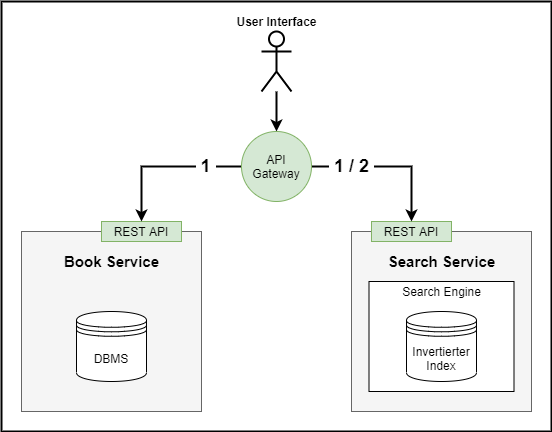
\includegraphics[width=0.6\linewidth]{images/direkte_aktualisierung.png}
    \caption{Datenpipeline: Direkte Aktualisierung}
    \label{fig:direkte_aktualisierung}
\end{figure}

\begin{description}
    \item[Vorteile:]\hfill \\
    Ein Vorteil bei dieser Art der Datenpipeline ist die \textbf{Datenaktualität} innerhalb der Search Engine. Da die CRUD-Befehle nicht nur in die Datenhaltung der Microservice, sondern auch zur Search Engine geschickt werden, findet eine ständige Synchronisation statt.
    
    Für die Datenpipeline werden keine zusätzlichen Softwarekomponenten benötigt und die Kommunikation mit den Datenbanksystemen findet über abstrahierte Schnittstellen der Services statt. Somit sind die Auswahlkriterien bezüglich der \textbf{Kompatibilität mit Datenbanksystemen und Softwarekomponenten von MCC} nicht von Bedeutung, da weder eine direkte Kommunikation mit einem Datenbanksystem, noch eine Verwendung von Softwarekomponenten vorhanden ist.
    
    \item[Nachteile:]\hfill \\
    Die Nachteile einer direkten Aktualisierung liegen beim \textbf{Mehraufwand für die Entwicklung} und Wartung von bestehenden oder neuen Funktionalitäten. Die Entwickler müssen gezielt die einzelnen CRUD-Befehle nicht nur an den eigentlichen Services sondern zusätzlich an den Search Services schicken.

    Ein weiteres Problem ist die \textbf{Datenkonsistenz zwischen Datenhaltung der Microservices und der Search Engine}, sobald eine Komponente des Systems ausfällt. Durch das parallele Benachrichtigen der Microservices und der Search Engine ist die Atomarität der Transaktionen nicht mehr gegeben.

    Bezüglich der \textbf{Auslastung des Systems} besteht bei dieser Art der Datenpipeline das Problem, dass bei jeder Aktion, welche einen CRUD-Befehl beinhaltet ein Nachrichtenaustausch mit dem Search Service stattfindet. Dadurch entsteht eine Engstelle in der Software, durch welche die Performance des gesamten Systems verlangsamt wird.

\end{description}

\subsection{Pull-or-Push Aktualisierung\label{subsec4.3.3:Unterunterpunkt-3}}

Eine weitere Umsetzungsmöglichkeit für die Datenpipeline ist die \glqq Pull-or-Push\grqq{} - Aktualisierung. Hier wird vom Benutzer lediglich die Aktualisierung der eigentlichen Datenhaltung initiiert. Zu einem definierten Zeitpunkt werden dann die bearbeiteten Daten entweder mit einem Pull-or-Push Mechanismus an den Search Service geschickt.

\begin{description}
    \item[Pull:]\hfill \\
    Die Search Service initiiert die Aktualisierung des invertierten Index nach einer vordefinierten Zeitspanne und holt sich dann die Datenänderungen aus den verschiedenen Microservices.
    
    \item[Push:]\hfill \\
    Nach einer vordefinierten Zeitspanne schicken die verschiedenen Microservices die Datenänderungen an die Search Engine, wo dann eine Aktualisierung des invertierten Index stattfinden kann.

\end{description}

In \autoref{fig:pullpush_aktualisierung} ist eine Darstellung der Pull-or-Push Aktualisierung abgebildet. Über das User Interface kann der Benutzer Aktionen initiieren, welche dann von den jeweiligen Microservices bearbeitet werden. Im Falle von CRUD-Befehlen werden lediglich die Datenhaltungsschichten der Microservices benötigt \footnote{In der \autoref{fig:pullpush_aktualisierung} durch eine \glqq 1\grqq{} markiert}. Die Aktualisierung des invertierten Indexes der Search Engine wird zu einem späteren Zeitpunk durch einen Pull- oder Push-Mechanismus durchgeführt \footnote{In der \autoref{fig:pullpush_aktualisierung} durch eine \glqq 2\grqq{} markiert}. Für das stellen einer Suchanfrage kann anschließend der Benutzer direkt mit dem Search Service interagieren \footnote{In der \autoref{fig:pullpush_aktualisierung} durch eine \glqq 3\grqq{} markiert}.

\begin{figure}[H]
    \centering
    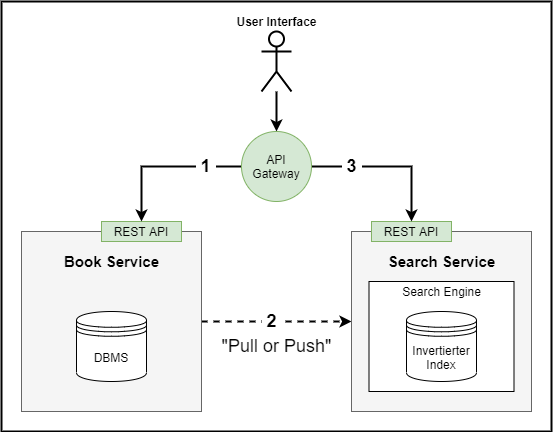
\includegraphics[width=0.6\linewidth]{images/pullpush_aktualisierung.png}
    \caption{Datenpipeline: Pull-or-Push Aktualisierung}
    \label{fig:pullpush_aktualisierung}
\end{figure}

\begin{description}
    \item[Vorteile:]\hfill \\
    Im Gegensatz zur direkten Aktualisierung gibt es bei der Pull-or-Push Aktualisierung keine Engstelle in der Software, da bei jeder Benutzeraktion lediglich die Datenhaltungen der Microservices beeinträchtigt werden. So entsteht durch diese Art der Datenpipeline nur eine minimale \textbf{Mehrbelastung des Systems}.

    Ein weiterer Vorteil ist die \textbf{Kompatibilität bezüglich den Datenbanksystemen und den Softwarekomponenten von MCC}, da hier über vordefinierte Schnittstellen kommuniziert wird.
    
    \item[Nachteile:]\hfill \\
    Ein großer Nachteil bei dieser Datenpipeline ist die \textbf{Datenaktualität} innerhalb der Search Engine. Die Datenaktualität ist dabei von der Zeitspanne des Pull-or-Push Mechanismus abhängig. So kann es bei der Bearbeitung einer Suchanfrage dazu kommen, dass die Search Engine zu dem Zeitpunkt noch nicht aktualisiert wurde und somit eine unvollständige Trefferliste erzeugt wird.

    Bei der Entwicklung und Wartung von neuen Funktionalitäten müssen die Entwickler bei den Pull-or-Push Mechanismen entscheiden, wann die Datenaktualisierung stattfinden soll. Dies resultiert in einen \textbf{Mehraufwand bei der Entwicklung}, da auch definiert werden muss, welche Teile des Datenkontextes \glqq durchsuchbar\grqq{} gemacht werden sollen.

\end{description}

\subsection{Change-Data-Capture Aktualisierung\label{subsec4.3.4:Unterunterpunkt-4}}

Neben der Umsetzungsmöglichkeit der direkten Aktualisierung und der Pull-or-Push Aktualisierung, gibt es noch die Umsetzungsmöglichkeit mithilfe des \gls{cdc} - Pattern. Bei CDC handelt es sich um ein Software Design Pattern, welches die Datenintegration zwischen einer Datenbank und deren Datenquellen definiert \cite{Datenbankenverstehen.de.2021}.

Durch das Beobachten von Datenänderungen in den Quelldatenbanken, ermöglicht \gls{cdc} ein Bewegen und Verarbeiten der Daten in nahezu Echtzeit \cite{JohnKutay.2021}. Somit können Datenreplikationen mit geringer Latenz erzeugt werden. Für die Umsetzung einer CDC-Datenpipeline gibt es vier gängige Methoden \cite{MarkVandeWiel.2021}:

\begin{description}
    \item[Zeitpunkt der letzten Aktualisierung:]\hfill \\
    Um hierbei die Datenbankänderungen mit CDC zu beobachten, müssen die Datenbanktabellen eine \glqq DATE\_MODIFIED\grqq{}-Spalte enthalten, welche den Zeitpunkt der letzten Änderung des Datensatzes protokolliert. Bei der Datensynchronisierung zwischen einer Zieldatenbank und den Quelldatenbanken filtert man nun mithilfe von CDC bezüglich einer solchen \glqq DATE\_MODIFIED\grqq{}-Spalte und entnimmt die Datenänderungen, welche seit der letzten Datenextraktion geändert wurden.

    Ein Problem bei diesem Vorgehen ist das Beobachten von Löschoperationen. Hierbei werden die Datensätze häufig komplett entfernt und ein Beobachten der Spalte \glqq DATE\_MODIFIED\grqq{} ist nicht mehr möglich.

    Auch muss solch eine Spalte für jede Datenbanktabelle zur Verfügung stehen und aktuell gehalten werden. Durch Datenbank-Trigger können diese Spalten aktuell gehalten werden, was jedoch einen erhöhten Overhead verursacht.

    \item[Tabellenunterschiede:]\hfill \\
    Eine weitere Möglichkeit für die Umsetzung einer CDC-Datenpipeline ist das regelmäßige Vergleichen der Tabellenunterschiede. Hierbei wird der aktuelle Zustand der Daten mit dem vorherigen Zustand verglichen.

    Im Vergleich zur Methode, bei welcher man auf die letzte Aktualisierung einer Zeile achtet, können hierbei auch die Löschoperationen berücksichtigt werden. Ein Nachteil ist der hohe Ressourcenverbrauch, welcher bei der Berechnung der Unterschiede zwischen den Datenbeständen entsteht. Somit kann die Methode der Tabellenunterschiede nicht in Echtzeit durchgeführt werden, da für eine ständige Durchführung zu viele Ressourcen benötigt werden.

    \item[Trigger-basierte CDC:]\hfill \\
    Mit der Verwendung von Datenbank-Triggern können Schattentabellen erzeugt werden, auf welchen dann die CDC-Datenpipeline die Änderungen erfassen kann. Hierbei gibt es die Möglichkeit die kompletten Datensätze in eine Schattentabelle zu speichern oder die Möglichkeit lediglich die Primärschlüssel der Datensätze in Verbindung mit der vorgenommen Art der Datenänderung (Einfügen, Aktualisieren oder Löschen) abzuspeichern.

    Bei der Variante der kompletten Speicherung der Datensätze in eine Schattentabelle, entsteht bei der Erstellung und Aktualisierung der Schattentabelle ein Overhead. Ein geringerer Overhead entsteht bei der Variante, wo lediglich die Primärschlüssel mit der Art der Datenänderung in die Schattentabelle gespeichert werden. Hierbei ist aber ein Join zur Quelltabelle nötig, sobald die Datenänderungen ausgelesen werden möchten.

    Somit senkt eine Trigger-basierte CDC-Datenpipeline den Aufwand für die Extraktion der Änderungen, erhöht aber den Aufwand für die Aufzeichnung der Änderungen in den Schattentabellen.

    \item[Log-basierte CDC:]\hfill \\
    Datenbanksysteme speichern alle Änderungen in einem Transaktionsprotokoll, um somit abgebrochene Transaktionen wieder rückgängig zu machen und um die Persistenz der Datenhaltung bei Ausfall des Datenbanksystems zu bewahren. Die Log-basierte CDC-Datenpipeline liest hierbei die Transaktionsprotokolle der Datenbanksysteme und entnimmt daraus die Datenänderungen.

    Ein Problem bei der Verwendung der Transaktionsprotokolle ist der fehlende Standard bezüglich der Art und Weise, wie Änderungen abgespeichert werden. So sind die Transaktionsprotokolle von verschiedenen Datenbankanbietern nach keinem Standart aufgebaut und unterscheiden sich stark voneinander.

\end{description}

Im Rahmen dieser Arbeit und den Umsetzungsmöglichkeiten einer Datenpipeline wird die Log-basierte CDC-Datenpipeline näher betrachtet. In \autoref{fig:changedatacapture_aktualisierung} ist eine Datenpipeline mit einer CDC-Aktualisierung abgebildet. Wie bereits bei der Pull-or-Push Aktualisierung initiiert der Benutzer über ein User Interface eine Aktion, welche dann vom jeweiligen Microservice bearbeitet wird. Werden dabei die Daten der jeweiligen Datenbank durch CRUD-Befehle bearbeitet, werden jene Änderungen auch in den Datenbank-spezifischen Transaktionsprotokollen festgehalten.

Durch die große Varianz der unterschiedlichen Transaktionsprotokolle ist eine eigene Implementierung solch einer CDC-Software umständlich. Abhilfe schafft das Open Source Framework \glqq Debezium\grqq{}, welche auf dem Log-basierten CDC arbeitet und die Änderungen der Transaktionsprotokolle beobachtet.

\begin{description}
\item[Debezium:]\hfill \\
    Nach Luber \cite{StefanLuber.2021} ist Debezium ein Open Source Framework, welches Änderungen in einer Datenbank erfasst und in Form von Event-Streams anderen Anwendungen zur Verfügung stellt. Debezium baut hierfür auf dem Framework \glqq Apache Kafka Connect\grqq{} auf, welches für die Implementierung von Kafka-Schnittstellen verantwortlich ist. Solche Schnittstellen werden entweder in Form von Quellkonnektoren oder Sink-Konnektoren umgesetzt und sind dafür zuständig Datensätze an Kafka zu schicken (Quellkonnektoren) oder Datensätze aus Kafka-Topics an andere Systeme (Sink-Konnektoren) weiterzuschicken \cite{DebeziumCommunity.2021b}.
    
    Debezium bietet derzeit für folgende Datenbankmanagementsysteme Kafka-Konnektoren an: \cite{DebeziumCommunity.2021}

    \begin{itemize}
        \item MongoDB
        \item MySQL
        \item PostgreSQL
        \item SQL Server
        \item Oracle
        \item Db2
    \end{itemize}

    Eine Vorabversion der Kafka-Konnektoren wird bereits für folgende Datenbankmanagementsysteme angeboten: \cite{DebeziumCommunity.2021}

    \begin{itemize}
        \item Cassandra
        \item Vitess
    \end{itemize}

    % \begin{figure}[H]
    %     \centering
    %     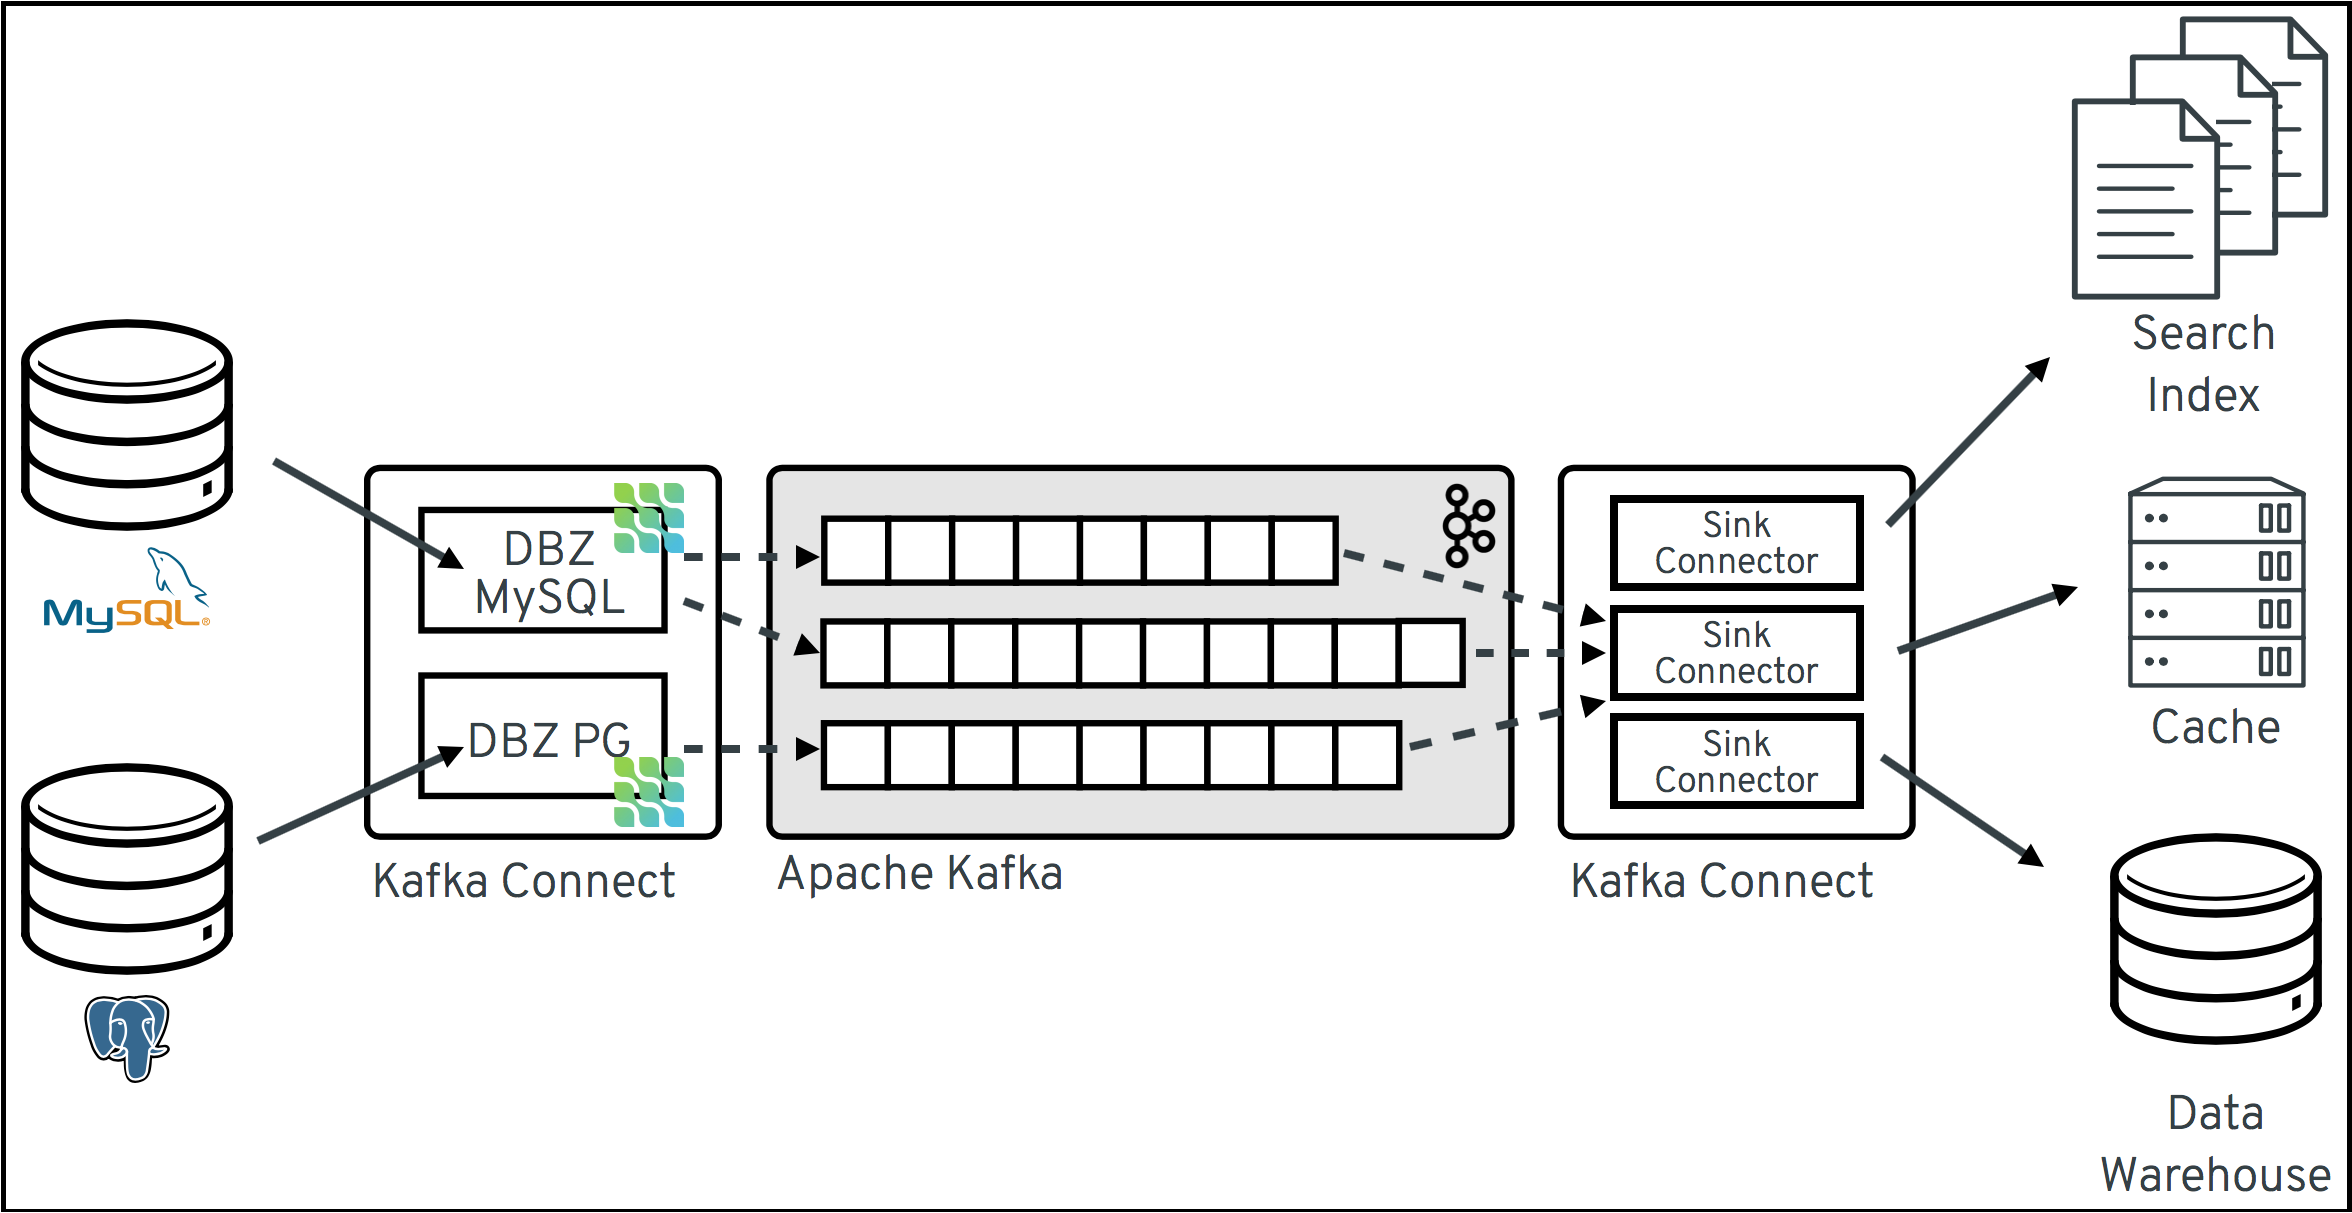
\includegraphics[width=0.9\linewidth]{images/debezium_kafka_pipeline.png}
    %     \caption{Architektur von Debezium}
    %     \label{fig:architektur_von_debezium}
    % \end{figure}

\end{description}

In \autoref{fig:changedatacapture_aktualisierung} ist die Verwendung von Debezium im Gesamtbild der Datenpipeline abgebildet. Zu erkennen ist, das Debezium auf die Transaktionsprotokolle der unterschiedlichen DBMS zugreift und dessen Änderungen an den Message Broker Apache Kafka weiterleitet. Somit fungiert Debezium als Kafka-Produzent und leitet die Datenänderungen aus den Quelldatenbanken an die entsprechenden Kafka-Topics weiter. Um die Daten aus den Kafka-Topics in die jeweilige Search Engine zu leiten, müssen geeignete Kafka-Sink-Konnektoren verwendet werden.

\begin{figure}[H]
    \centering
    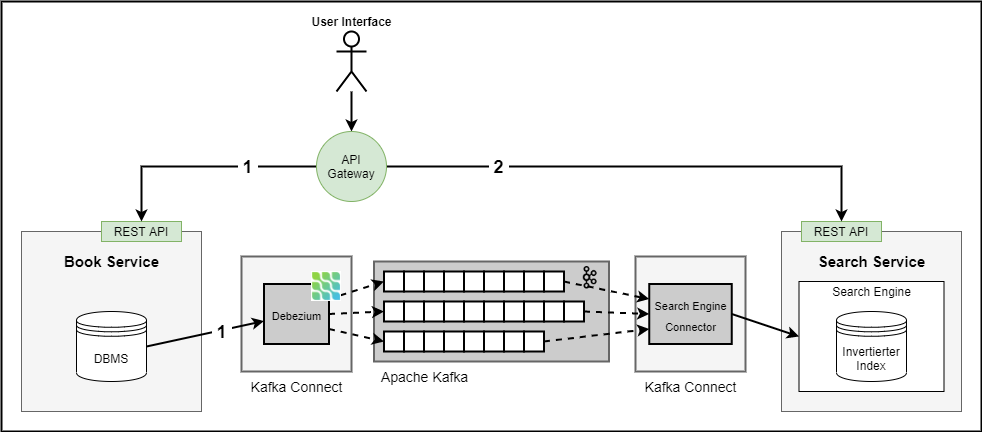
\includegraphics[width=0.9\linewidth]{images/CDC_aktualisierung.png}
    \caption{Datenpipeline: Change-Data-Capture Aktualisierung}
    \label{fig:changedatacapture_aktualisierung}
\end{figure}

\begin{description}
    \item[Vorteile:]\hfill \\
    Ein Vorteil bei der Verwendung der CDC-Aktualisierung liegt bei der Echtzeit der Daten in der jeweiligen Search Engine. Grund dafür ist die stetige Überwachung der DBMS-spezifischen Transaktionsprotokolle.
    
    \item[Nachteile:]\hfill \\
    Text

\end{description}

\subsection{Vergleich\label{subsec4.3.5:Unterunterpunkt-5}}

Inhalt

\section{Gesamtkonzept\label{sec4.4:Unterpunkt-4}}

Inhalt

% \begin{figure}[H]
%     \centering
%     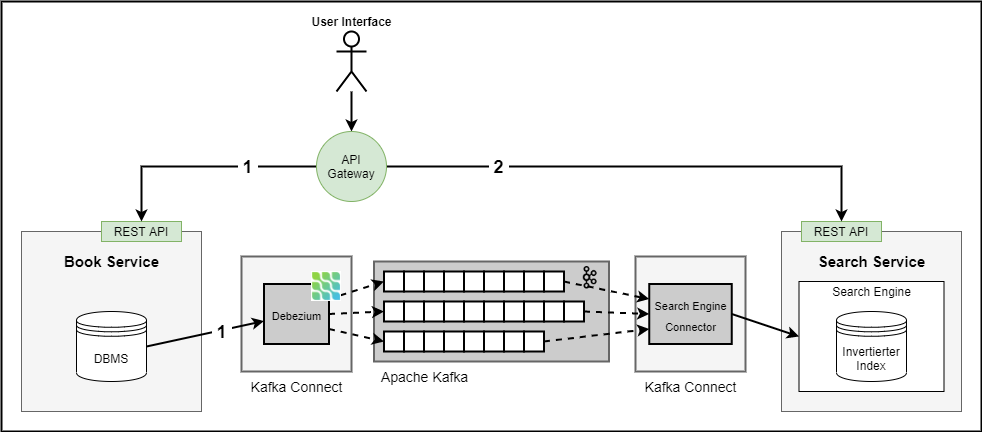
\includegraphics[width=0.9\linewidth]{images/CDC_aktualisierung.png}
%     \caption{Datenpipeline: Change-Data-Capture Aktualisierung}
%     \label{fig:changedatacapture_aktualisierung}
% \end{figure}
\chapter{Prototypische Umsetzung\label{chap5:Fuenftes-Kapitel}}

Inhalt

\section{Client\label{sec5.1:Unterpunkt-1}}

Inhalt

\section{Search Service\label{sec5.2:Unterpunkt-2}}

Inhalt

\section{Anbindung an Apache Kafka\label{sec5.3:Unterpunkt-3}}

Inhalt
\chapter{Fazit und Ausblick\label{chap6:Sechstes-Kapitel}}

In folgendem Kapitel sollen die Ergebnisse aus dem theoretischen Abschnitt, als auch aus dem praktischen Abschnitt dargelegt werden. Darauffolgend wird ein Ausblick auf die tatsächliche Integrierung in das Produktionsleitsystem MCC gegeben.

\section{Fazit\label{sec6.1:Unterpunkt-1}}

Die Ergebnisse der vorliegenden Arbeit können in einen theoretischen und einen praktischen Abschnitt unterteilt werden.

\subsubsection{Theoretischer Abschnitt}

In dem theoretischen Abschnitt wurde auf die unterschiedlichen Umsetzungsmöglichkeiten für eine Suchfunktionalität in modernen Informationssystemen eingegangen. Erläutert wurden dabei die Umsetzungsmöglichkeiten \glqq Volltextsuche\grqq{}, \glqq facettierte Suche\grqq{} und \glqq semantische Suche\grqq{}. Ebenso wurde durch das \glqq TF-IDF\grqq{}-Modell eine Vorgehensweise für die Relevanzbestimmung aufgezeigt. Mithilfe einer Relevanzbestimmung können die Suchtreffer sortiert werden, so das relevante Ergebnisse dem Benutzer priorisiert angezeigt werden.

Durch das Aufzeigen von allgemeingültigen Architektur-Prinzipien und im spezielleren Anti-Pattern der Microservice-Architektur, wurde eine theoretische Grundlage für das Vermeiden von monolithischen Seiteneffekten aufgezeigt. Jenes Verständnis ist Grundlage für die Integration einer Suchfunktionalität, beziehungsweise einer Search Engine, in einer Microservice-Umgebung.

Für die spätere Integrierung in das Produktionsleitsystem MCC, wurde in \autoref{chap3:Drittes-Kapitel} der Funktionsumfang von MCC aufgezeigt. Näher vorgestellt wurden dabei die Funktionalitäten der Schichten \glqq MCC Platform\grqq{}, \glqq Core Services - Production\grqq{}, \glqq SCADA\grqq{} und \glqq PCS\grqq{}. Für die vorgestellten Umsetzungsmöglichkeiten einer Suchfunktionalität, wurden die jeweiligen Umfänge anhand des Produktionsleitsystem MCC definiert.

\subsubsection{Praktischer Abschnitt}

Der praktische Teil der vorliegenden Arbeit wurde durch eine Konzeption, bezüglich der Integrierung einer Suchfunktionalität in das Produktionsleitsystem MCC, begonnen. Als Komponenten des endgültigen Gesamtkonzeptes wurde die Auswahl einer Search Engine und die Auswahl einer geeigneten Datenpipeline durchgeführt.

Für die Pflege des Datenbestandes einer Search Engine, wurde eine geeignete Datenpipeline gesucht. Miteinander verglichen wurden die Umsetzungsmöglichkeiten \glqq Dual Write Aktualisierung\grqq{}, \glqq Polling Aktualisierung\grqq{} und \glqq Change-Data-Capture Aktualisierung\grqq{}. Anhand vordefinierter Vergleichskriterien wurde sich schlussendlich für die Umsetzungsmöglichkeit der CDC-Aktualisierung entschieden. Hierbei entstehen für die spätere Entwicklung und Wartung von neuen Funktionalitäten nur minimale Mehrbelastungen. Ebenso werden die Datenänderungen in unterschiedlichsten Datenquellen durch CDC-Software, wie zum Beispiel \glqq Debezium\grqq{}, registriert und an einen Message Broker weitergeleitet.

Nach der Festlegung von Vergleichskriterien für die Auswahl einer Search Engine, wurden die Search Engines \glqq Apache Solr\grqq{} und \glqq Elasticsearch\grqq{} miteinander verglichen. Da beide auf der Programmbibliothek \glqq Apache Lucene\grqq{} aufbauen, wurde hierfür ein theoretischer Einblick gegeben. Für die prototypische Umsetzung wurde sich schlussendlich für die Search Engine Elasticsearch entschieden, da diese eine offizielle Schnittstelle mit dem Message Broker Kafka besitzt.

Abgeschlossen wurde die Phase der Konzeption mit dem Erläutern eines Gesamtkonzeptes für die prototypische Umsetzung.

Innerhalb der prototypischen Umsetzung wurde eine Bibliothek mit integrierter Volltextsuche umgesetzt. Mit Hilfe der Bibliothek besteht die Möglichkeit Bücher anzulegen, zu bearbeiten und zu entfernen. Über eine CDC-Datenpipeline werden die Datenänderungen aus der MongoDB an die Search Engine Elasticsearch geschickt. Durch den Aufruf von Elasticsearch kann in der Bibliothek eine Volltextsuche zur Verfügung gestellt werden.

\section{Ausblick\label{sec6.2:Unterpunkt-2}}

Für die spätere Integrierung in das Produktionsleitsystem MCC gilt es noch einige weitere Themenfelder näher zu betrachten. Sowohl die Kafka-Konnektoren von Debezium als auch die Search Engine sind für die horizontale Skalierung geeignet. Dies wurde jedoch bei der Umsetzung des Prototypen noch nicht berücksichtigt, sodass hierbei noch Recherchearbeit bezüglich den Konfigurationsmöglichkeiten notwendig ist.

Auch gibt es derzeit bei der Firma Enisco Bemühungen eine Streaming Base in MCC einzubauen. Durch jene Komponente soll es möglich sein verschiedene Transaktionen zu unterschiedlichen Datenquellen in größere Transaktionen zu gruppieren. Sollte demnach eine Teiltransaktion nicht erfolgreich beendet werden, werde auch die Änderungen der anderen Teiltranskationen rückgängig gemacht. Durch dieses Vorgehen wäre eine Schwachstelle der \glqq Dual Write Aktualisierung\grqq{} beseitigt. Es gilt demnach eine erneute Bewertung durchzuführen, ob die vorgeschlagene \glqq CDC-Aktualisierung\grqq{} immer noch die beste Wahl ist, mit dem Hintergedanken, dass durch die Verwendung einer \glqq Dual Write Aktualisierung\grqq{} eine Engstelle im System erzeugt wird.

Weitere Nachforschung bedarf es bei der Umsetzung einer facettierten Suche in MCC. Hierbei gilt es zu untersuchen, inwiefern die vorgestellten Search Engines für solch eine Suche geeignet sind und welche Konfigurationsmöglichkeiten vorhanden sind. Zu berücksichtigen ist zu dem die Art und Weiße wie Datenänderungen, zusammen mit den jeweiligen Metadaten, erkannt und an die Search Engine weitergegeben werden.

    \newpage
    \bibliographystyle{citation/alphadin}
    \addcontentsline{toc}{chapter}{\bibname}
    \bibliography{bibtex-daten/T3000.bib} 

\end{document}